\documentclass[10pt]{article}

\usepackage[utf8]{inputenc}
\usepackage[T1]{fontenc}
\usepackage{lmodern}
\usepackage[margin=0.72in]{geometry}
\usepackage{graphicx}
\usepackage{booktabs}
\usepackage{longtable}
\usepackage{tabularx}
\usepackage{array}
\usepackage{float}
\usepackage{placeins}
\usepackage{pdflscape}
\usepackage{subcaption}
\usepackage{xcolor}
\usepackage{microtype}
\usepackage{enumitem}
\usepackage{fancyhdr}
\usepackage[colorlinks=true,linkcolor=blue,urlcolor=blue,hypertexnames=false]{hyperref}
\renewcommand{\thetable}{S\arabic{table}}
\renewcommand{\thefigure}{S\arabic{figure}}

\graphicspath{{figures/}}
\setlength{\parindent}{0pt}
\setlength{\parskip}{0.45em}
\setlength{\tabcolsep}{4pt}
\renewcommand{\arraystretch}{1.10}
\setlength{\emergencystretch}{3em}
\pagestyle{fancy}
\fancyhf{}
\lhead{Additional file 1}
\rhead{Major-revision supplementary material}
\cfoot{\thepage}

\begin{document}

\begin{titlepage}
\centering
{\Large\bfseries Additional file 1\par}
\vspace{0.35cm}
{\LARGE\bfseries Supplementary methods, tables, and figures\par}
\vspace{0.8cm}
{\large Supplement to:\par}
\vspace{0.2cm}
{\Large\bfseries Multi-Modal Molecular Representation Learning Prioritizes Class I HDAC Inhibitors\par}
{\Large\bfseries for Pan-Cancer Transcriptomic Reversal\par}
\vspace{0.8cm}
{\large Siyuan Tong, Wen Zhang, and Shiliang Ji\par}
\vfill
\begin{minipage}{0.88\textwidth}
\small
\textbf{Evidence policy.} This supplement distinguishes predicted reversal, measured LINCS transcriptomic reversal, biological context, and structural sensitivity. Measured reversal is not a viability assay; reversal-associated genes are not asserted direct drug targets; DepMap knockout effects are not compound responses; and docking is not binding validation. The 24 tables below are compact human-readable views. Full, filterable rows and source fields are supplied in Additional file 2.
\end{minipage}
\vfill
{\large Evidence freeze: 19 July 2026\par}
\end{titlepage}

\tableofcontents
\clearpage

\section{Scope, corrections, and candidate policy}

The revision uses three completed computational evidence packages: (E1) official-condition measured LINCS comparison and prediction--measurement concordance; (E2) biological reanalysis after candidate roles were frozen, including networks, pathways, and DepMap Public 26Q1; and (E3) controlled zinc-aware docking with crystallographic redocking, a designed zinc-chelation decoy, and receptor sensitivity. A direct external drug-sensitivity package was conditional on candidate-matched public data and was not performed because such data were unavailable for TC-H-106. No new wet-lab experiment is claimed.

The candidate hierarchy was frozen before network, pathway, dependency, and docking interpretation. Mocetinostat is the core computational candidate; NCH-51 is secondary; TC-H-106 is exploratory/original-method-sensitive; RG2833 is prediction-only because no measured LINCS signature was found; and Tianeptinaline/BG-1010 is excluded from primary inference because official identifier resolution exposed a name--structure conflict. Belinostat, PCI-24781, and Panobinostat provide class support; Entinostat and Vorinostat are reference controls.

The revised package removes simulated TCGA survival and stage analyses, unsupported tumor-mutation-burden conclusions, proxy DeepCE/ChemCPA claims, unsupported legacy ablation values, GDSC surrogate ``validation,'' direct-target language for reversed genes, and MMFF94 energy claims as thermodynamic evidence. A pre-correction HDAC holdout is retained only as provenance; all model inference uses the corrected annotation-defined 1,856-profile, 30-structure holdout.

\section{Dataset, model scope, and leakage-aware evaluation}

Table S1 separates signatures, perturbagen tokens, nominal conditions, canonical structures, and cell lines. This distinction prevents the 55,695 modeling rows from being described as unique compounds or biological replicates.

\begingroup
\small
\begin{table}[H]
\centering
\caption{Composition of the quality-controlled LINCS modeling dataset and frozen screening library. Level 5 signatures are not unique compounds or raw biological replicates.}
\label{tab:s_dataset}
\begin{tabular}{@{}p{0.30\textwidth}rp{0.58\textwidth}@{}}
\toprule
Item & Count & Interpretation \\
\midrule
Level 5 signatures & 55,695 & Modeling rows after quality control \\
Signature-ID perturbagen tokens & 13,314 & Includes instance suffixes \\
Base perturbagen identifiers & 11,527 & Normalized BRD identifiers \\
Unique canonical structures & 11,445 & Valid RDKit structures \\
Cell lines & 65 & Across the modeling dataset \\
Perturbagen-token--cell combinations & 39,266 & Descriptive combinations \\
Perturbagen-token--cell--time--dose conditions & 52,834 & Nominal conditions \\
Additional signatures beyond nominal conditions & 2,861 & Plate/batch-level Level 5 entries \\
Expression genes & 12,328 & Shared disease/perturbation feature space \\
Screened canonical compounds & 28,477 & Frozen screening library; distinct from the modeling structures \\
\bottomrule
\end{tabular}
\end{table}
\endgroup


Both neural predictors are chemical-structure-only models. They do not receive cell-line identity, dose, or time. Their output is therefore a structure-conditioned central tendency across training conditions, not a condition-specific response. Leave-cell-line evaluation measures agreement with profiles from held-out cellular backgrounds under this formulation; it does not show that the models learned cell-specific response rules.

\begingroup
\small
\begin{table}[H]
\centering
\caption{Frozen model, optimization, and interpretation settings.}
\label{tab:s_settings}
\begin{tabular}{@{}p{0.25\textwidth}p{0.70\textwidth}@{}}
\toprule
Item & Frozen specification \\
\midrule
Prediction input & Canonical chemical structure only; no cell-line, dose, or time covariates \\
Target & 12,328-gene LINCS Level 5 perturbation vector \\
Atom stream & 43-dimensional element identity; 3 Transformer layers; 512 pooled dimensions; no bond adjacency \\
Fingerprint stream & 1,024-bit radius-2 Morgan fingerprint; 512-dimensional projection \\
Dual-stream parameters & 38,682,152 \\
Fingerprint MLP parameters & 28,415,016 \\
Optimization & MSE; AdamW; learning rate 2e-4; weight decay 1e-4; batch 128 \\
Stopping & Maximum 30 epochs; patience 5; checkpoint by validation MSE \\
Benchmark seeds & Pair split 1--5; other splits 1--3; grouping seed 42 \\
Primary screening metrics & signed wTRS and negative Spearman disease--perturbation correlation \\
Stability configurations & 48 primary; 72 only when legacy wTRS is added as sensitivity \\
\bottomrule
\end{tabular}
\end{table}
\endgroup


The split audit first checks signature identifiers and then distinguishes exact-structure and scaffold exposure. Zero scaffold overlap is required only for the scaffold split. The corrected annotation-defined HDAC holdout requires zero exact HDAC structure overlap; 11 scaffolds remain shared and are reported rather than mislabeled as leakage.

\begingroup
\scriptsize
\begin{table}[H]
\centering
\caption{Leakage and structural-overlap audit. Exact-structure overlap is zero for leave-drug, scaffold, and corrected annotation-defined HDAC evaluations; the scaffold column is the directly recorded Murcko overlap.}
\label{tab:s_split}
\begin{tabular}{@{}lrrrrrr@{}}
\toprule
Split & Train n & Test n & Train struct. & Test struct. & Sig. ovlp. & Scaffold ovlp. \\
\midrule
Drug--cell pair & 47,376 & 8,319 & 10,582 & 3,827 & 0 & 2,489 \\
Leave drug out & 47,728 & 7,967 & 9,728 & 1,717 & 0 & 686 \\
Leave cell line out & 50,520 & 5,175 & 11,170 & 2,826 & 0 & 1,914 \\
Scaffold split & 47,851 & 7,844 & 9,831 & 1,614 & 0 & 0 \\
Corrected annotation-defined HDAC & 53,839 & 1,856 & 11,415 & 30 & 0 & 11 \\
\bottomrule
\end{tabular}
\end{table}
\endgroup


\begin{landscape}
\begingroup
\scriptsize
\begin{table}[H]
\centering
\caption{Generalization summary as mean (seed SD). Corrected 1,856-profile HDAC runs replace stale pre-correction summaries.}
\label{tab:s_model_summary}
\begin{tabular}{@{}llrrrrrrr@{}}
\toprule
Split & Model & Seeds & Test & MSE & MAE & $R^2$ & Pearson & Spearman \\
\midrule
Corrected annotation-defined HDAC holdout & Dual stream & 3 & 1856 & 1.326 (0.026) & 0.839 (0.005) & 0.131 (0.017) & 0.378 (0.009) & 0.345 (0.010) \\
Corrected annotation-defined HDAC holdout & Fingerprint MLP & 3 & 1856 & 1.333 (0.015) & 0.841 (0.004) & 0.127 (0.010) & 0.379 (0.007) & 0.344 (0.006) \\
Leave cell line out & Dual stream & 3 & 5175 & 0.942 (0.004) & 0.714 (0.000) & 0.121 (0.003) & 0.266 (0.010) & 0.243 (0.010) \\
Leave cell line out & Fingerprint MLP & 3 & 5175 & 0.941 (0.007) & 0.713 (0.002) & 0.122 (0.006) & 0.272 (0.010) & 0.249 (0.010) \\
Leave drug out & Dual stream & 3 & 7967 & 0.919 (0.003) & 0.717 (0.001) & 0.052 (0.003) & 0.188 (0.000) & 0.166 (0.001) \\
Leave drug out & Fingerprint MLP & 3 & 7967 & 0.919 (0.001) & 0.716 (0.001) & 0.052 (0.001) & 0.191 (0.003) & 0.170 (0.003) \\
Drug--cell pair & Dual stream & 5 & 8319 & 0.882 (0.004) & 0.704 (0.003) & 0.108 (0.004) & 0.259 (0.009) & 0.237 (0.009) \\
Drug--cell pair & Fingerprint MLP & 5 & 8319 & 0.881 (0.001) & 0.703 (0.001) & 0.110 (0.002) & 0.263 (0.005) & 0.241 (0.005) \\
Scaffold split & Dual stream & 3 & 7844 & 0.973 (0.000) & 0.738 (0.002) & 0.062 (0.000) & 0.185 (0.006) & 0.163 (0.007) \\
Scaffold split & Fingerprint MLP & 3 & 7844 & 0.971 (0.002) & 0.736 (0.001) & 0.064 (0.002) & 0.186 (0.001) & 0.165 (0.002) \\
\bottomrule
\end{tabular}
\end{table}
\endgroup
\end{landscape}


\begin{landscape}
\begingroup
\scriptsize
\begin{longtable}{@{}llrrrrrrrrr@{}}
\caption{All 34 frozen model runs. Runtime includes training and evaluation on the recorded RTX 4090 environment.}\label{tab:s_runs}\\
\toprule
Split & Model & Seed & Test & Epoch & Runtime s & MSE & MAE & $R^2$ & Pearson & Spearman \\
\midrule
\endfirsthead
\multicolumn{11}{l}{\textit{Table continued}}\\
\toprule
Split & Model & Seed & Test & Epoch & Runtime s & MSE & MAE & $R^2$ & Pearson & Spearman \\
\midrule
\endhead
\midrule
\multicolumn{11}{r}{\textit{Continued on next page}}\\
\endfoot
\bottomrule
\endlastfoot
Corrected HDAC & Dual & 1 & 1,856 & 4 & 260.5 & 1.320 & 0.837 & 0.135 & 0.381 & 0.348 \\
Corrected HDAC & Dual & 2 & 1,856 & 5 & 282.7 & 1.355 & 0.845 & 0.112 & 0.385 & 0.353 \\
Corrected HDAC & Dual & 3 & 1,856 & 8 & 365.0 & 1.305 & 0.834 & 0.145 & 0.368 & 0.334 \\
Corrected HDAC & Fingerprint & 1 & 1,856 & 2 & 54.1 & 1.347 & 0.844 & 0.118 & 0.387 & 0.351 \\
Corrected HDAC & Fingerprint & 2 & 1,856 & 5 & 72.5 & 1.336 & 0.842 & 0.125 & 0.373 & 0.338 \\
Corrected HDAC & Fingerprint & 3 & 1,856 & 4 & 70.3 & 1.316 & 0.837 & 0.138 & 0.378 & 0.344 \\
Leave cell & Dual & 1 & 5,175 & 6 & 209.5 & 0.938 & 0.713 & 0.125 & 0.259 & 0.236 \\
Leave cell & Dual & 2 & 5,175 & 7 & 212.4 & 0.945 & 0.713 & 0.118 & 0.261 & 0.238 \\
Leave cell & Dual & 3 & 5,175 & 15 & 394.8 & 0.942 & 0.714 & 0.121 & 0.277 & 0.254 \\
Leave cell & Fingerprint & 1 & 5,175 & 13 & 78.9 & 0.937 & 0.712 & 0.125 & 0.277 & 0.254 \\
Leave cell & Fingerprint & 2 & 5,175 & 7 & 58.4 & 0.949 & 0.715 & 0.115 & 0.261 & 0.238 \\
Leave cell & Fingerprint & 3 & 5,175 & 15 & 91.5 & 0.937 & 0.711 & 0.126 & 0.279 & 0.256 \\
Leave drug & Dual & 1 & 7,967 & 2 & 132.4 & 0.916 & 0.716 & 0.055 & 0.187 & 0.165 \\
Leave drug & Dual & 2 & 7,967 & 4 & 163.5 & 0.921 & 0.718 & 0.049 & 0.188 & 0.166 \\
Leave drug & Dual & 3 & 7,967 & 5 & 182.0 & 0.921 & 0.717 & 0.050 & 0.188 & 0.167 \\
Leave drug & Fingerprint & 1 & 7,967 & 5 & 48.5 & 0.918 & 0.716 & 0.053 & 0.195 & 0.173 \\
Leave drug & Fingerprint & 2 & 7,967 & 2 & 36.7 & 0.919 & 0.715 & 0.052 & 0.188 & 0.167 \\
Leave drug & Fingerprint & 3 & 7,967 & 5 & 51.7 & 0.920 & 0.716 & 0.051 & 0.191 & 0.169 \\
Pair & Dual & 1 & 8,319 & 13 & 327.2 & 0.880 & 0.702 & 0.111 & 0.268 & 0.246 \\
Pair & Dual & 2 & 8,319 & 5 & 191.6 & 0.888 & 0.707 & 0.102 & 0.248 & 0.225 \\
Pair & Dual & 3 & 8,319 & 14 & 336.4 & 0.877 & 0.701 & 0.113 & 0.268 & 0.245 \\
Pair & Dual & 4 & 8,319 & 8 & 237.8 & 0.881 & 0.704 & 0.109 & 0.256 & 0.233 \\
Pair & Dual & 5 & 8,319 & 10 & 278.0 & 0.885 & 0.705 & 0.106 & 0.258 & 0.236 \\
Pair & Fingerprint & 1 & 8,319 & 14 & 86.7 & 0.881 & 0.703 & 0.109 & 0.268 & 0.246 \\
Pair & Fingerprint & 2 & 8,319 & 11 & 71.9 & 0.879 & 0.702 & 0.112 & 0.263 & 0.241 \\
Pair & Fingerprint & 3 & 8,319 & 6 & 55.0 & 0.883 & 0.704 & 0.108 & 0.254 & 0.232 \\
Pair & Fingerprint & 4 & 8,319 & 14 & 87.5 & 0.881 & 0.703 & 0.110 & 0.266 & 0.244 \\
Pair & Fingerprint & 5 & 8,319 & 10 & 72.7 & 0.880 & 0.702 & 0.111 & 0.263 & 0.240 \\
Scaffold & Dual & 1 & 7,844 & 2 & 135.6 & 0.973 & 0.735 & 0.062 & 0.179 & 0.156 \\
Scaffold & Dual & 2 & 7,844 & 4 & 167.6 & 0.974 & 0.739 & 0.061 & 0.191 & 0.170 \\
Scaffold & Dual & 3 & 7,844 & 3 & 152.6 & 0.974 & 0.739 & 0.061 & 0.186 & 0.163 \\
Scaffold & Fingerprint & 1 & 7,844 & 6 & 56.7 & 0.974 & 0.736 & 0.062 & 0.187 & 0.165 \\
Scaffold & Fingerprint & 2 & 7,844 & 3 & 45.2 & 0.969 & 0.735 & 0.066 & 0.185 & 0.163 \\
Scaffold & Fingerprint & 3 & 7,844 & 3 & 44.7 & 0.971 & 0.736 & 0.064 & 0.186 & 0.166 \\
\end{longtable}
\endgroup
\end{landscape}


\begingroup
\footnotesize
\begin{longtable}{@{}llrrrrr@{}}
\caption{Paired model differences. Positive values favor the dual stream; all intervals include zero except the candidate-specific PCI-24781 comparison reported separately.}\label{tab:s_paired}\\
\toprule
Split & Metric & Seeds & Dual advantage & SD & 95\% low & 95\% high \\
\midrule
\endfirsthead
\multicolumn{7}{l}{\textit{Table continued}}\\
\toprule
Split & Metric & Seeds & Dual advantage & SD & 95\% low & 95\% high \\
\midrule
\endhead
\midrule
\multicolumn{7}{r}{\textit{Continued on next page}}\\
\endfoot
\bottomrule
\endlastfoot
Pair & MSE & 5 & -0.001 & 0.006 & -0.009 & 0.006 \\
Pair & MAE & 5 & -0.001 & 0.003 & -0.005 & 0.003 \\
Pair & R2 & 5 & -0.001 & 0.006 & -0.009 & 0.006 \\
Pair & Pearson & 5 & -0.003 & 0.011 & -0.017 & 0.010 \\
Pair & Spearman & 5 & -0.003 & 0.011 & -0.018 & 0.011 \\
Leave drug & MSE & 3 & -0.001 & 0.002 & -0.006 & 0.005 \\
Leave drug & MAE & 3 & -0.002 & 0.001 & -0.005 & 0.002 \\
Leave drug & R2 & 3 & -0.001 & 0.002 & -0.006 & 0.005 \\
Leave drug & Pearson & 3 & -0.003 & 0.004 & -0.013 & 0.006 \\
Leave drug & Spearman & 3 & -0.004 & 0.004 & -0.013 & 0.005 \\
Leave cell & MSE & 3 & -0.001 & 0.004 & -0.012 & 0.010 \\
Leave cell & MAE & 3 & -0.001 & 0.002 & -0.006 & 0.005 \\
Leave cell & R2 & 3 & -0.001 & 0.004 & -0.011 & 0.009 \\
Leave cell & Pearson & 3 & -0.007 & 0.010 & -0.031 & 0.018 \\
Leave cell & Spearman & 3 & -0.006 & 0.010 & -0.031 & 0.018 \\
Scaffold & MSE & 3 & -0.002 & 0.003 & -0.009 & 0.004 \\
Scaffold & MAE & 3 & -0.002 & 0.003 & -0.009 & 0.004 \\
Scaffold & R2 & 3 & -0.002 & 0.003 & -0.009 & 0.004 \\
Scaffold & Pearson & 3 & -0.001 & 0.007 & -0.018 & 0.016 \\
Scaffold & Spearman & 3 & -0.002 & 0.008 & -0.022 & 0.018 \\
Corrected HDAC & MSE & 3 & 0.006 & 0.023 & -0.051 & 0.064 \\
Corrected HDAC & MAE & 3 & 0.002 & 0.005 & -0.010 & 0.014 \\
Corrected HDAC & R2 & 3 & 0.004 & 0.015 & -0.034 & 0.042 \\
Corrected HDAC & Pearson & 3 & -0.001 & 0.011 & -0.030 & 0.027 \\
Corrected HDAC & Spearman & 3 & 0.001 & 0.013 & -0.030 & 0.032 \\
\end{longtable}
\endgroup


Across generalization settings, the fingerprint MLP was slightly better on average in the pair, leave-drug, leave-cell-line, and scaffold evaluations. The corrected HDAC holdout was mixed by metric and every paired interval included zero. These tables replace all proxy state-of-the-art comparisons and do not support dual-stream superiority.

\begin{landscape}
\section{Candidate identity, condition coverage, and corrected holdout}

\begingroup
\scriptsize
\begin{table}[H]
\centering
\caption{Candidate identity, BRD identifier, and frozen evidence role. Tianeptinaline/BG-1010 is retained only to document the identity conflict.}
\label{tab:s_identity}
\begin{tabular}{@{}p{2.8cm}p{2.8cm}p{4.2cm}ccp{7.5cm}@{}}
\toprule
Candidate & BRD ID & Frozen role & HDAC annotated & Name conflict & Interpretation \\
\midrule
Mocetinostat & BRD-K16485616 & core candidate & yes & no & Primary computational hypothesis \\
TC-H-106 & BRD-K45044657 & exploratory / original-method-sensitive & yes & no & Limited HiQ coverage; close training neighbor \\
NCH-51 & BRD-K52522949 & secondary candidate & yes & no & Measured support; scaffold-exposure caveat \\
Belinostat & BRD-K17743125 & class support & yes & no & Measured HDAC-class support \\
PCI-24781 & BRD-K12867552 & class support & yes & no & Measured HDAC-class support \\
Panobinostat & BRD-K02130563 & class support & yes & no & Measured HDAC-class support \\
Entinostat & BRD-K77908580 & reference control & yes & no & Established HDAC reference \\
Vorinostat & BRD-K81418486 & reference control & yes & no & Established HDAC reference \\
RG2833 & BRD-K02389548 & prediction only & yes & no & No measured LINCS profile \\
Tianeptinaline / BG-1010 & BRD-A73972952 & identity conflict; excluded & no & yes & Name--structure conflict; exact training exposure \\
\bottomrule
\end{tabular}
\end{table}
\endgroup


\begingroup
\scriptsize
\begin{table}[H]
\centering
\caption{Official LINCS condition and quality coverage. ``All cells'' and ``HiQ cells'' are deliberately separated.}
\label{tab:s_coverage}
\begin{tabular}{@{}lrrrrrlrrr@{}}
\toprule
Candidate & All & QC & HiQ & All cells & HiQ cells & Times h & Dose levels & Min $\mu$M & Max $\mu$M \\
\midrule
Mocetinostat & 14 & 8 & 8 & 12 & 8 & 6 | 24 & 1 & 10.000 & 10.000 \\
NCH-51 & 17 & 8 & 8 & 10 & 8 & 6 | 24 & 1 & 10.000 & 10.000 \\
TC-H-106 & 6 & 4 & 4 & 5 & 4 & 6 | 24 & 1 & 10.000 & 10.000 \\
Belinostat & 24 & 13 & 12 & 12 & 6 & 6 | 24 & 4 & 0.370 & 10.000 \\
PCI-24781 & 19 & 13 & 13 & 13 & 10 & 6 | 24 & 1 & 10.000 & 10.000 \\
Panobinostat & 126 & 93 & 84 & 15 & 10 & 6 | 24 & 20 & 0.001 & 10.000 \\
Entinostat & 101 & 77 & 67 & 14 & 10 & 6 | 24 & 13 & 0.040 & 10.000 \\
Vorinostat & 899 & 521 & 487 & 54 & 35 & 6 | 24 | 48 & 38 & 0.001 & 30.000 \\
Tianeptinaline/BG-1010 & 6 & 1 & 1 & 2 & 1 & 6 | 24 & 1 & 10.000 & 10.000 \\
\bottomrule
\end{tabular}
\end{table}
\endgroup

\end{landscape}

The official LINCS cell count and the HiQ-eligible official-cell count are separate fields in Table S8. This resolves the earlier ambiguity in which a single ``Cells'' column could refer to either the full official metadata or the primary HiQ analysis.

\begingroup
\small
\begin{table}[H]
\centering
\caption{Pre-correction versus corrected annotation-defined HDAC holdout. The pre-correction row is provenance only and is excluded from inference.}
\label{tab:s_prepost}
\begin{tabular}{@{}lrrrrr@{}}
\toprule
Version & Test profiles & Test structures & Test cells & $\Delta$ profiles & $\Delta$ structures \\
\midrule
discarded\_pre\_fix & 1,565 & 21 & 55 & 0 & 0 \\
corrected\_final & 1,856 & 30 & 55 & 291 & 9 \\
\bottomrule
\end{tabular}
\end{table}
\endgroup


The correction added nine annotation-defined structures and 291 profiles. NCH-51 was removed from training and placed into the final test set. Table S10 provides the complete compound-level inventory rather than only an aggregate count.

\begingroup
\footnotesize
\begin{longtable}{@{}lllrrlll@{}}
\caption{Complete 30-structure corrected annotation-defined HDAC holdout inventory.}\label{tab:s_hdac30}\\
\toprule
BRD ID & Compound & Profiles & Cells & Annotation source & Added by fix & NCH-51 removed \\
\midrule
\endfirsthead
\multicolumn{7}{l}{\textit{Table continued}}\\
\toprule
BRD ID & Compound & Profiles & Cells & Annotation source & Added by fix & NCH-51 removed \\
\midrule
\endhead
\midrule
\multicolumn{7}{r}{\textit{Continued on next page}}\\
\endfoot
\bottomrule
\endlastfoot
BRD-K85133207 & HDAC1-selective & 50 & 11 & metadata & yes & no \\
BRD-K29313308 & HDAC3-selective & 55 & 11 & metadata & yes & no \\
BRD-K76698671 & HNHA & 8 & 7 & metadata & yes & no \\
BRD-K69840642 & ISOX & 48 & 43 & metadata & yes & no \\
BRD-K83837640 & JNJ-26481585 & 11 & 9 & metadata\_and\_audit & no & no \\
BRD-K45528773 & M-344 & 6 & 3 & audit & no & no \\
BRD-K04466929 & Merck60 & 51 & 8 & metadata\_and\_audit & no & no \\
BRD-K52522949 & NCH-51 & 17 & 11 & metadata & yes & yes \\
BRD-K13169950 & NSC-3852 & 20 & 14 & metadata\_and\_audit & no & no \\
BRD-K12867552 & PCI-24781 & 19 & 13 & metadata\_and\_audit & no & no \\
BRD-K88742110 & PCI-34051 & 43 & 11 & metadata\_and\_audit & no & no \\
BRD-K45044657 & TC-H-106 & 6 & 5 & audit & no & no \\
BRD-K74761218 & WT-171 & 15 & 11 & metadata & yes & no \\
BRD-A63989068 & apicidin & 6 & 3 & metadata & yes & no \\
BRD-K64606589 & apicidin & 85 & 14 & metadata & yes & no \\
BRD-K17743125 & belinostat & 24 & 12 & metadata\_and\_audit & no & no \\
BRD-K56957086 & dacinostat & 27 & 12 & metadata\_and\_audit & no & no \\
BRD-K11558771 & droxinostat & 9 & 8 & metadata\_and\_audit & no & no \\
BRD-K77908580 & entinostat & 101 & 14 & metadata\_and\_audit & no & no \\
BRD-K13810148 & givinostat & 5 & 4 & metadata\_and\_audit & no & no \\
BRD-K16485616 & mocetinostat & 14 & 12 & metadata\_and\_audit & no & no \\
BRD-K02130563 & panobinostat & 126 & 15 & metadata\_and\_audit & no & no \\
BRD-K67102207 & phenylbutyrate & 6 & 6 & audit & no & no \\
BRD-K11663430 & pyroxamide & 13 & 10 & audit & no & no \\
BRD-K22503835 & scriptaid & 38 & 14 & metadata\_and\_audit & no & no \\
BRD-K52313696 & tacedinaline & 83 & 11 & audit & no & no \\
BRD-K98426715 & tubacin & 7 & 6 & metadata & yes & no \\
BRD-K00627859 & tubastatin-a & 51 & 8 & metadata\_and\_audit & no & no \\
BRD-K41260949 & valproic-acid & 13 & 6 & metadata\_and\_audit & no & no \\
BRD-K81418486 & vorinostat & 899 & 55 & metadata\_and\_audit & no & no \\
\end{longtable}
\endgroup


\begingroup
\small
\begin{table}[H]
\centering
\caption{Strict leave-drug candidate membership.}
\label{tab:s_ldo_member}
\begin{tabular}{@{}lrrrr@{}}
\toprule
Candidate & Train & Test & Test cells & Strict LDO \\
\midrule
Belinostat & 24 & 0 & 0 & no \\
Entinostat & 101 & 0 & 0 & no \\
Mocetinostat & 0 & 14 & 12 & yes \\
NCH-51 & 17 & 0 & 0 & no \\
PCI-24781 & 0 & 19 & 13 & yes \\
Panobinostat & 126 & 0 & 0 & no \\
RG2833 & 0 & 0 & 0 & no \\
TC-H-106 & 6 & 0 & 0 & no \\
Tianeptinaline/BG-1010 & 6 & 0 & 0 & no \\
Vorinostat & 899 & 0 & 0 & no \\
\bottomrule
\end{tabular}
\end{table}
\endgroup
\begingroup
\scriptsize
\begin{table}[H]
\centering
\caption*{Supplementary Table S11 (continued). Strict leave-drug candidate metrics. Only Mocetinostat and PCI-24781 were true test candidates.}
\begin{tabular}{@{}llrrrrrrr@{}}
\toprule
Candidate & Model & Seeds & Profiles & Cells & Pearson & 95\% low & 95\% high & Spearman \\
\midrule
Mocetinostat & dual\_stream & 3 & 14 & 12 & 0.483 & 0.393 & 0.574 & 0.476 \\
Mocetinostat & fingerprint\_mlp & 3 & 14 & 12 & 0.504 & 0.468 & 0.539 & 0.499 \\
PCI-24781 & dual\_stream & 3 & 19 & 13 & 0.308 & 0.152 & 0.464 & 0.270 \\
PCI-24781 & fingerprint\_mlp & 3 & 19 & 13 & 0.540 & 0.423 & 0.657 & 0.493 \\
\bottomrule
\end{tabular}
\end{table}
\endgroup


Only Mocetinostat and PCI-24781 satisfy strict leave-drug candidate membership. PCI-24781 significantly favored the fingerprint baseline for profile correlations; no strict candidate result favors the dual stream.

\section{Measured LINCS reversal and prediction--measurement concordance}

Measured profiles were aggregated hierarchically: median within candidate--dose--time--official-cell condition, median across conditions within official cell, comparison with each cancer disease vector, and summary across official cells and cancers. The HiQ stratum is primary; QC-pass and all-profile rows are sensitivity analyses.

\begin{landscape}
\begingroup
\scriptsize
\begin{table}[H]
\centering
\caption{Corrected-HDAC predicted versus HiQ measured reversal with 10,000 candidate--cancer crossed bootstrap iterations (seed 20260719).}
\label{tab:s_twoway}
\begin{tabular}{@{}llrrrrrrrr@{}}
\toprule
Metric & Model & Candidates & Cancers & Pearson & 95\% low & 95\% high & Spearman & 95\% low & 95\% high \\
\midrule
signed\_wtrs & dual\_stream & 8 & 22 & 0.642 & 0.365 & 0.838 & 0.640 & 0.297 & 0.840 \\
signed\_wtrs & fingerprint\_mlp & 8 & 22 & 0.805 & 0.601 & 0.911 & 0.803 & 0.554 & 0.919 \\
spearman\_reversal & dual\_stream & 8 & 22 & 0.813 & 0.634 & 0.919 & 0.801 & 0.594 & 0.909 \\
spearman\_reversal & fingerprint\_mlp & 8 & 22 & 0.853 & 0.710 & 0.921 & 0.830 & 0.653 & 0.910 \\
\bottomrule
\end{tabular}
\end{table}
\endgroup
\end{landscape}


The crossed bootstrap independently resampled eight candidates and 22 cancers. This is more conservative than treating 176 candidate--cancer pairs as independent. Leave-one-candidate-out and leave-one-cancer-out influence tables are in Additional file 2 and retain positive associations.

\begingroup
\footnotesize
\begin{longtable}{@{}llrrrrrr@{}}
\caption{Primary official-condition HiQ measured reversal across 22 cancer signatures.}\label{tab:s_measured}\\
\toprule
Candidate & Metric & HiQ & HiQ cells & Median & Q1 & Q3 & Positive cancers \% \\
\midrule
\endfirsthead
\multicolumn{8}{l}{\textit{Table continued}}\\
\toprule
Candidate & Metric & HiQ & HiQ cells & Median & Q1 & Q3 & Positive cancers \% \\
\midrule
\endhead
\midrule
\multicolumn{8}{r}{\textit{Continued on next page}}\\
\endfoot
\bottomrule
\endlastfoot
Belinostat & signed\_wtrs & 12 & 6 & 0.140 & 0.105 & 0.200 & 95.5 \\
Belinostat & spearman\_reversal & 12 & 6 & 0.058 & 0.037 & 0.092 & 95.5 \\
Entinostat & signed\_wtrs & 67 & 10 & 0.082 & 0.041 & 0.101 & 95.5 \\
Entinostat & spearman\_reversal & 67 & 10 & 0.082 & 0.038 & 0.100 & 95.5 \\
Mocetinostat & signed\_wtrs & 8 & 8 & 0.262 & 0.172 & 0.316 & 95.5 \\
Mocetinostat & spearman\_reversal & 8 & 8 & 0.137 & 0.088 & 0.151 & 95.5 \\
NCH-51 & signed\_wtrs & 8 & 8 & 0.194 & 0.144 & 0.249 & 95.5 \\
NCH-51 & spearman\_reversal & 8 & 8 & 0.103 & 0.068 & 0.133 & 95.5 \\
PCI-24781 & signed\_wtrs & 13 & 10 & 0.139 & 0.111 & 0.211 & 95.5 \\
PCI-24781 & spearman\_reversal & 13 & 10 & 0.075 & 0.057 & 0.107 & 95.5 \\
Panobinostat & signed\_wtrs & 84 & 10 & 0.191 & 0.152 & 0.224 & 95.5 \\
Panobinostat & spearman\_reversal & 84 & 10 & 0.061 & 0.035 & 0.095 & 95.5 \\
TC-H-106 & signed\_wtrs & 4 & 4 & 0.119 & 0.081 & 0.160 & 90.9 \\
TC-H-106 & spearman\_reversal & 4 & 4 & 0.113 & 0.071 & 0.158 & 90.9 \\
Vorinostat & signed\_wtrs & 487 & 35 & 0.054 & 0.036 & 0.122 & 95.5 \\
Vorinostat & spearman\_reversal & 487 & 35 & 0.043 & 0.024 & 0.080 & 95.5 \\
\end{longtable}
\endgroup


\begin{figure}[H]
\centering
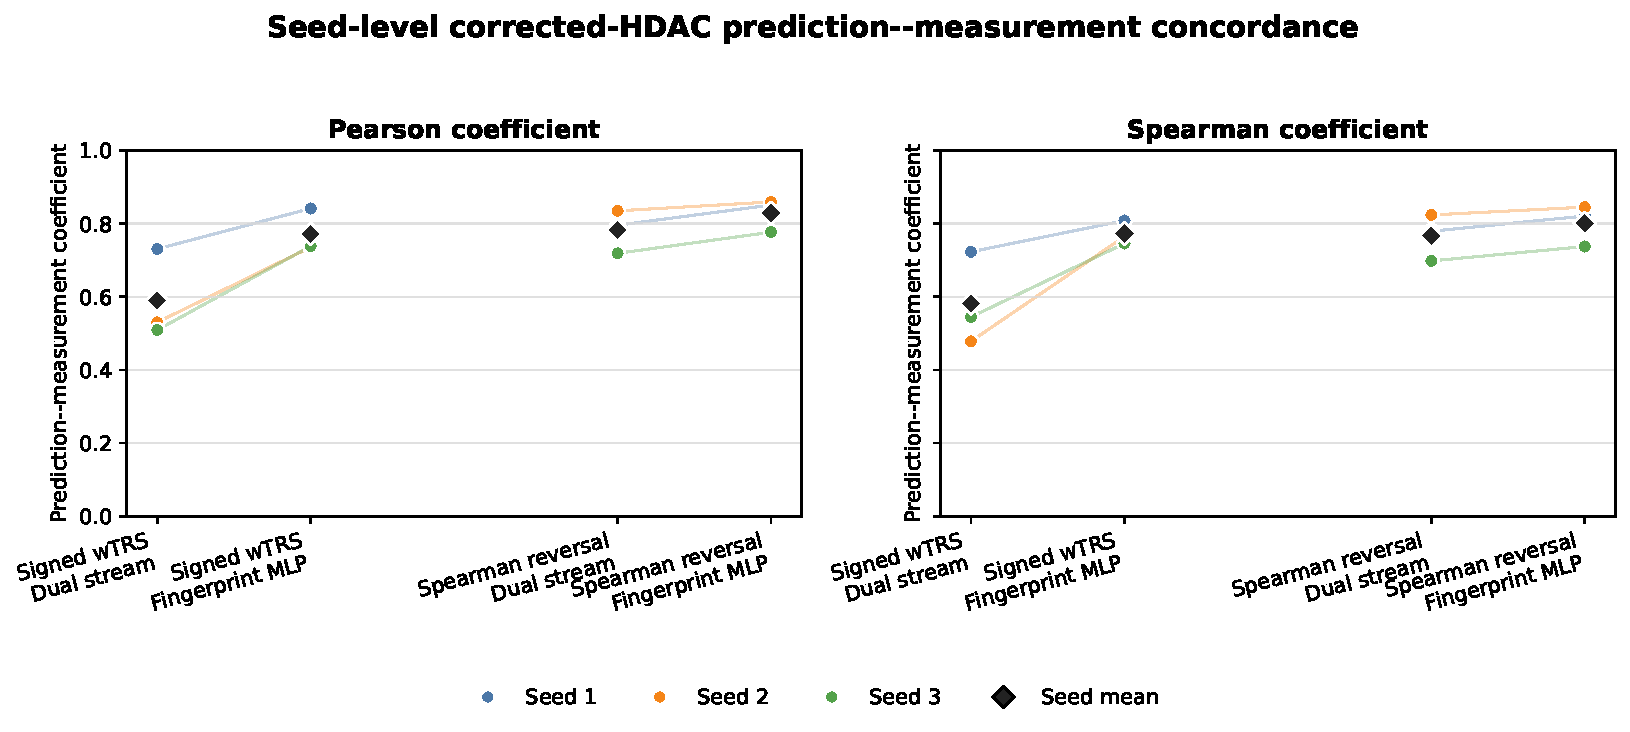
\includegraphics[width=0.96\textwidth]{predicted_measured_seed_variability.pdf}
\caption{\textbf{Seed-level prediction--measurement concordance.} Pearson and Spearman coefficients are shown separately for every corrected annotation-defined HDAC seed, model, and primary reversal definition. Large markers denote seed means. The figure exposes run-to-run variability that is summarized by the crossed candidate--cancer intervals in the main text; it is not a second independent validation dataset.}
\end{figure}

\begin{landscape}
\centering
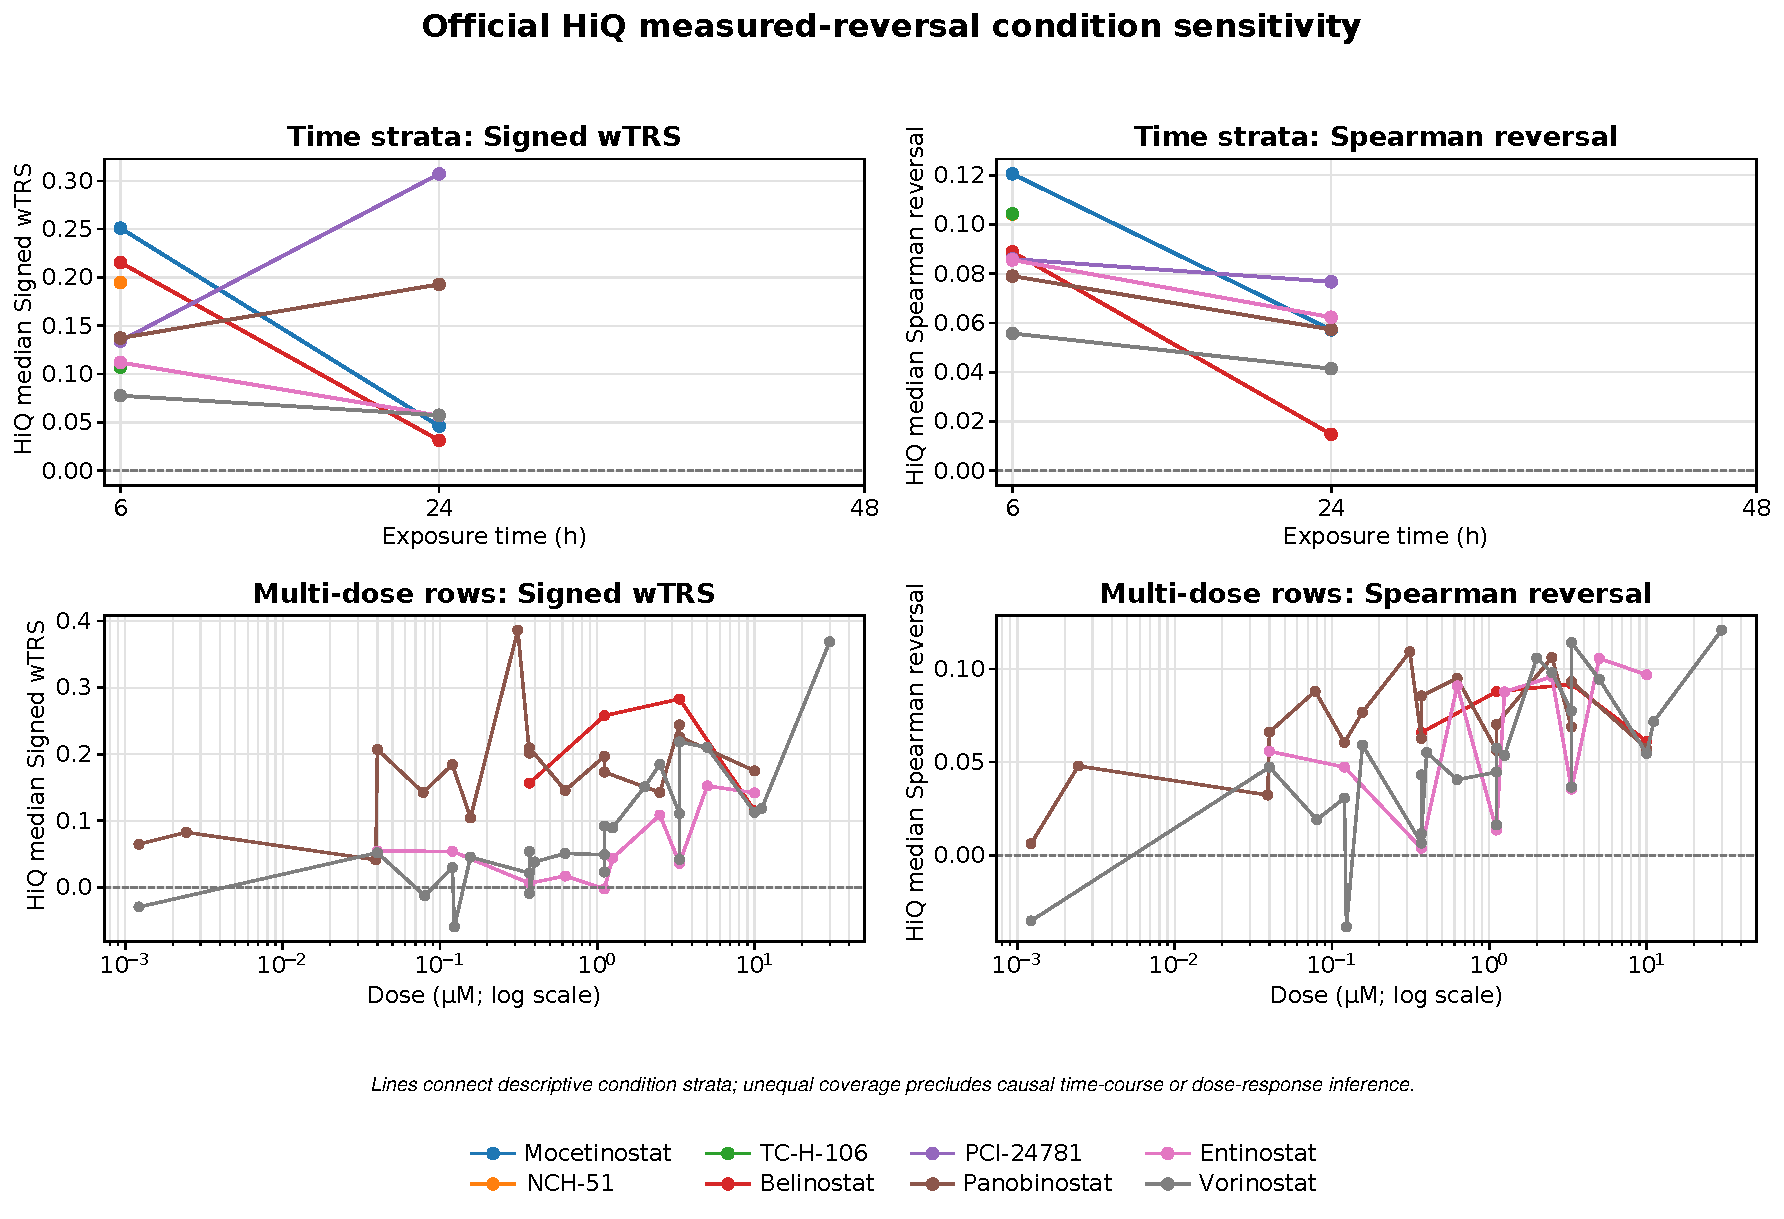
\includegraphics[height=4.85in,keepaspectratio]{measured_condition_sensitivity.pdf}
\captionof{figure}{\textbf{Measured LINCS time- and dose-stratum sensitivity.} HiQ pan-cancer median signed wTRS and Spearman reversal are shown by exposure time for the eight primary compounds and by dose for the four reference or class-support compounds with more than one profiled dose. Unequal cells, signatures, and condition coverage prevent causal dose--response or time-course interpretation; these panels are descriptive sensitivity checks.}
\vspace{0.25em}
\begin{minipage}{0.96\linewidth}
\small
All eight primary compounds had positive median measured reversal under signed and rank-based definitions. These are experimental expression responses, not direct drug-sensitivity, target-engagement, or efficacy measurements. The all-profile comparison against 11,445 canonical compounds in Additional file 2 is unmatched for dose, time, cell, and quality and is therefore not a condition-matched non-HDAC null.
\end{minipage}
\end{landscape}

\begin{landscape}
\section{Candidate stability, structural exposure, and formal class enrichment}
The primary stability hierarchy contains 48 configurations: four generalization or distribution-shift regimes, two models, three seeds, and two primary reversal metrics. Adding the legacy reversal-only magnitude score produces 72 configurations and is explicitly sensitivity analysis. These regime labels do not imply that every named candidate is unseen under every configuration. Candidate identity and training exposure override descriptive rank; this is why the high-ranking identity-conflicted Tianeptinaline/BG-1010 row remains excluded.

\begingroup
\scriptsize
\begin{table}[H]
\centering
\caption{Candidate stability under the 48-configuration primary hierarchy and 72-configuration legacy-inclusive sensitivity analysis.}
\label{tab:s_stability}
\begin{tabular}{@{}llrrrrrr@{}}
\toprule
Candidate & Role & Primary n & Primary median & Primary worst & Sensitivity n & Sensitivity median & $\Delta$ primary--sens. \\
\midrule
Belinostat & class\_support & 48 & 70.0 & 56.8 & 72 & 92.8 & -22.8 \\
Entinostat & reference\_control & 48 & 77.9 & 16.3 & 72 & 66.2 & 11.7 \\
Mocetinostat & core\_candidate & 48 & 92.2 & 53.8 & 72 & 91.9 & 0.3 \\
NCH-51 & secondary\_candidate & 48 & 88.5 & 65.6 & 72 & 95.4 & -6.9 \\
PCI-24781 & class\_support & 48 & 57.6 & 32.3 & 72 & 57.6 & 0.0 \\
Panobinostat & class\_support & 48 & 60.6 & 33.5 & 72 & 94.2 & -33.5 \\
RG2833 & prediction\_only & 48 & 72.0 & 47.4 & 72 & 57.3 & 14.7 \\
TC-H-106 & original\_method\_sensitive & 48 & 84.3 & 49.1 & 72 & 74.7 & 9.6 \\
Tianeptinaline/BG-1010 & identity\_conflict\_excluded & 48 & 90.0 & 71.0 & 72 & 76.7 & 13.3 \\
Vorinostat & reference\_control & 48 & 69.5 & 19.0 & 72 & 76.7 & -7.2 \\
\bottomrule
\end{tabular}
\end{table}
\endgroup


\begingroup
\tiny
\begin{table}[H]
\centering
\caption{Corrected annotation-defined HDAC structural-neighbor and scaffold exposure audit.}
\label{tab:s_neighbor}
\begin{tabular}{@{}p{3.2cm}p{3.7cm}rrrrrrrr@{}}
\toprule
Candidate & Role & Train & Test & Max Tanimoto & Top-10 mean & Exact train & Scaffold train & Same-scaffold n & Conflict \\
\midrule
Mocetinostat & core candidate & 0 & 14 & 0.537 & 0.447 & no & no & 0 & no \\
TC-H-106 & exploratory / original-method-sensitive & 0 & 6 & 0.789 & 0.438 & no & no & 0 & no \\
NCH-51 & secondary candidate & 0 & 17 & 0.431 & 0.366 & no & yes & 1 & no \\
Belinostat & class support & 0 & 24 & 0.500 & 0.339 & no & yes & 8 & no \\
PCI-24781 & class support & 0 & 19 & 0.410 & 0.317 & no & no & 0 & no \\
Panobinostat & class support & 0 & 126 & 0.381 & 0.315 & no & yes & 1 & no \\
Entinostat & reference control & 0 & 101 & 0.558 & 0.429 & no & no & 0 & no \\
Vorinostat & reference control & 0 & 899 & 0.697 & 0.503 & no & yes & 296 & no \\
RG2833 & prediction only & 0 & 0 & 0.574 & 0.407 & no & no & 0 & no \\
Tianeptinaline/BG-1010 & identity conflict; excluded & 6 & 0 & 1.000 & 0.508 & yes & yes & 1 & yes \\
\bottomrule
\end{tabular}
\end{table}
\endgroup

\end{landscape}

\begin{landscape}
\centering
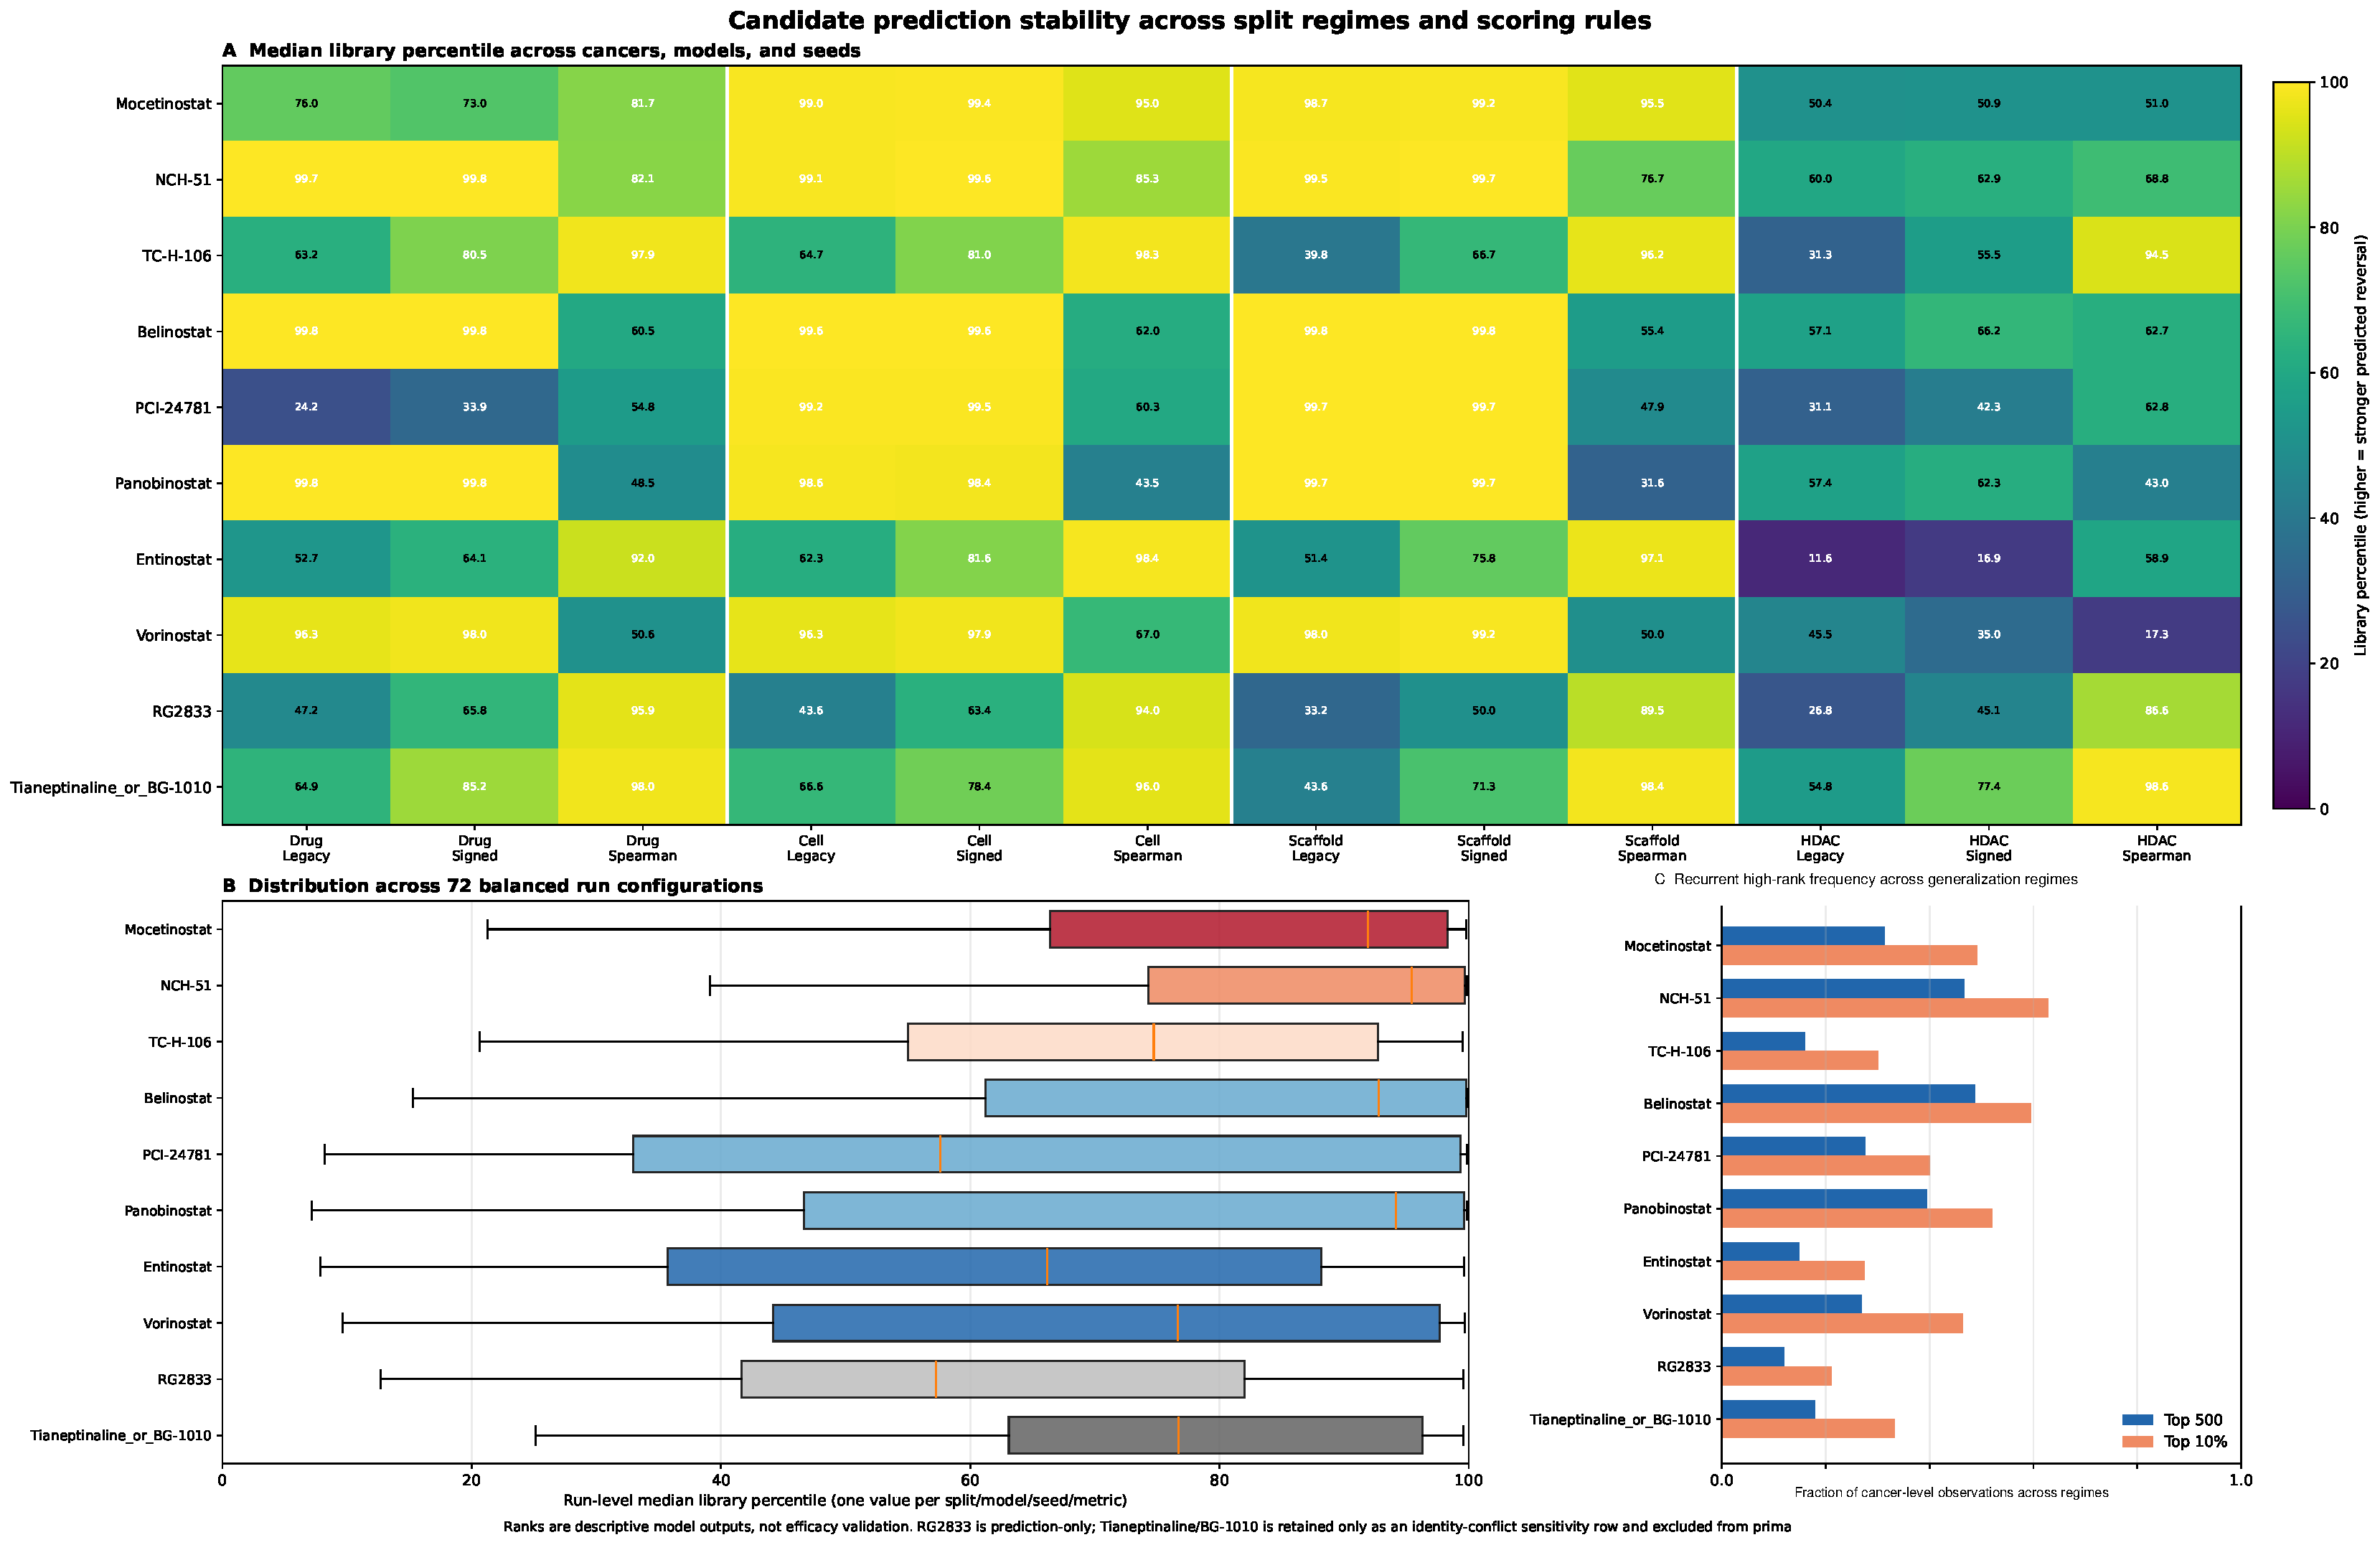
\includegraphics[width=0.96\linewidth,keepaspectratio]{candidate_stability_expanded_72.pdf}
\captionof{figure}{\textbf{Expanded split- and metric-level candidate stability sensitivity.} The heatmap reports the full 72-configuration legacy-inclusive audit by split and reversal definition, with run-level distributions and recurrent high-rank frequencies. This expands, rather than repeats, the 48-configuration primary summary in main Figure 4. Legacy wTRS remains a sensitivity metric and does not determine candidate eligibility.}
\end{landscape}

\begin{landscape}
\begingroup
\scriptsize
\begin{longtable}{@{}llrrrrrrrr@{}}
\caption{Formal HDAC enrichment at fixed revision library cutoffs. Consensus ranks equally average 24 screening runs across 22 cancers per compound; Fisher tests are one-sided and FDR is within each metric and annotation definition.}\label{tab:s_enrichment}\\
\toprule
Metric & Definition & Top fraction & Top k & Library HDAC & Observed & Expected & Fold & $P$ & FDR \\
\midrule
\endfirsthead
\multicolumn{10}{l}{\textit{Table continued}}\\
\toprule
Metric & Definition & Top fraction & Top k & Library HDAC & Observed & Expected & Fold & $P$ & FDR \\
\midrule
\endhead
\midrule
\multicolumn{10}{r}{\textit{Continued on next page}}\\
\endfoot
\bottomrule
\endlastfoot
signed\_wtrs & annotation\_defined\_HDAC & 0.5 & 143 & 39 & 4 & 0.20 & 20.42 & 4.37e-05 & 5.83e-05 \\
signed\_wtrs & annotation\_defined\_HDAC & 1.0 & 285 & 39 & 5 & 0.39 & 12.81 & 4.22e-05 & 5.83e-05 \\
signed\_wtrs & annotation\_defined\_HDAC & 5.0 & 1,424 & 39 & 11 & 1.95 & 5.64 & 2.16e-06 & 8.62e-06 \\
signed\_wtrs & annotation\_defined\_HDAC & 10.0 & 2,848 & 39 & 13 & 3.90 & 3.33 & 6.48e-05 & 6.48e-05 \\
signed\_wtrs & explicit\_class\_I\_target & 0.5 & 143 & 26 & 4 & 0.13 & 30.64 & 8.36e-06 & 8.36e-06 \\
signed\_wtrs & explicit\_class\_I\_target & 1.0 & 285 & 26 & 5 & 0.26 & 19.22 & 5.37e-06 & 7.16e-06 \\
signed\_wtrs & explicit\_class\_I\_target & 5.0 & 1,424 & 26 & 11 & 1.30 & 8.46 & 1.81e-08 & 7.25e-08 \\
signed\_wtrs & explicit\_class\_I\_target & 10.0 & 2,848 & 26 & 12 & 2.60 & 4.61 & 2.47e-06 & 4.93e-06 \\
spearman\_reversal & annotation\_defined\_HDAC & 0.5 & 143 & 39 & 1 & 0.20 & 5.11 & 1.78e-01 & 3.50e-01 \\
spearman\_reversal & annotation\_defined\_HDAC & 1.0 & 285 & 39 & 2 & 0.39 & 5.12 & 5.80e-02 & 2.32e-01 \\
spearman\_reversal & annotation\_defined\_HDAC & 5.0 & 1,424 & 39 & 3 & 1.95 & 1.54 & 3.09e-01 & 3.50e-01 \\
spearman\_reversal & annotation\_defined\_HDAC & 10.0 & 2,848 & 39 & 5 & 3.90 & 1.28 & 3.50e-01 & 3.50e-01 \\
spearman\_reversal & explicit\_class\_I\_target & 0.5 & 143 & 26 & 1 & 0.13 & 7.66 & 1.23e-01 & 4.60e-01 \\
spearman\_reversal & explicit\_class\_I\_target & 1.0 & 285 & 26 & 1 & 0.26 & 3.84 & 2.30e-01 & 4.60e-01 \\
spearman\_reversal & explicit\_class\_I\_target & 5.0 & 1,424 & 26 & 2 & 1.30 & 1.54 & 3.76e-01 & 4.90e-01 \\
spearman\_reversal & explicit\_class\_I\_target & 10.0 & 2,848 & 26 & 3 & 2.60 & 1.15 & 4.90e-01 & 4.90e-01 \\
\end{longtable}
\endgroup
\end{landscape}


\begin{landscape}
\section{Frozen reversal-associated genes, pathways, and networks}
Candidate roles were frozen before these analyses. At the 70\% primary consensus threshold, the top 200 reversal-associated genes per candidate/control were carried forward. The term ``reversal-associated'' is used because gene selection derives from the same disease--perturbation opposition used for ranking; these genes are not direct pharmacological targets.

\begingroup
\footnotesize
\begin{table}[H]
\centering
\caption{Frozen reversal-associated gene definition and mapping coverage. Selection precedes network and pathway interpretation.}
\label{tab:s_genedef}
\begin{tabular}{@{}llrrrrrr@{}}
\toprule
Candidate & Role & Threshold & Eligible & Stable direction & Top selected & STRING mappable & Mapping \% \\
\midrule
Mocetinostat & core\_candidate & 70.0 & 1,212 & 1,212 & 200 & 200 & 100.0 \\
NCH-51 & secondary\_candidate & 70.0 & 1,242 & 1,242 & 200 & 200 & 100.0 \\
TC-H-106 & exploratory\_candidate & 70.0 & 1,324 & 1,324 & 200 & 200 & 100.0 \\
Belinostat & class\_support & 70.0 & 1,167 & 1,167 & 200 & 200 & 100.0 \\
Entinostat & reference\_control & 70.0 & 880 & 880 & 200 & 200 & 100.0 \\
Vorinostat & reference\_control & 70.0 & 1,035 & 1,035 & 200 & 200 & 100.0 \\
\bottomrule
\end{tabular}
\end{table}
\endgroup


\input{generated/table_S18}
\end{landscape}

\begingroup
\footnotesize
\begin{longtable}{@{}lllr@{}}
\caption{Scope of significant g:Profiler results by candidate, reversal direction, and ontology/source.}\label{tab:s_path_scope}\\
\toprule
Candidate & Gene-set scope & Source & Significant terms \\
\midrule
\endfirsthead
\multicolumn{4}{l}{\textit{Table continued}}\\
\toprule
Candidate & Gene-set scope & Source & Significant terms \\
\midrule
\endhead
\midrule
\multicolumn{4}{r}{\textit{Continued on next page}}\\
\endfoot
\bottomrule
\endlastfoot
Belinostat & all\_selected & GO:BP & 167 \\
Belinostat & all\_selected & GO:CC & 44 \\
Belinostat & all\_selected & GO:MF & 4 \\
Belinostat & all\_selected & KEGG & 2 \\
Belinostat & all\_selected & REAC & 50 \\
Belinostat & disease\_down\_drug\_up & GO:BP & 7 \\
Belinostat & disease\_up\_drug\_down & GO:BP & 272 \\
Belinostat & disease\_up\_drug\_down & GO:CC & 75 \\
Belinostat & disease\_up\_drug\_down & GO:MF & 68 \\
Belinostat & disease\_up\_drug\_down & KEGG & 7 \\
Belinostat & disease\_up\_drug\_down & REAC & 100 \\
Entinostat & all\_selected & GO:BP & 182 \\
Entinostat & all\_selected & GO:CC & 56 \\
Entinostat & all\_selected & GO:MF & 31 \\
Entinostat & all\_selected & KEGG & 5 \\
Entinostat & all\_selected & REAC & 93 \\
Entinostat & disease\_down\_drug\_up & GO:BP & 7 \\
Entinostat & disease\_down\_drug\_up & GO:CC & 17 \\
Entinostat & disease\_down\_drug\_up & KEGG & 1 \\
Entinostat & disease\_down\_drug\_up & REAC & 1 \\
Entinostat & disease\_up\_drug\_down & GO:BP & 281 \\
Entinostat & disease\_up\_drug\_down & GO:CC & 111 \\
Entinostat & disease\_up\_drug\_down & GO:MF & 106 \\
Entinostat & disease\_up\_drug\_down & KEGG & 9 \\
Entinostat & disease\_up\_drug\_down & REAC & 146 \\
Mocetinostat & all\_selected & GO:BP & 163 \\
Mocetinostat & all\_selected & GO:CC & 30 \\
Mocetinostat & all\_selected & GO:MF & 2 \\
Mocetinostat & all\_selected & KEGG & 2 \\
Mocetinostat & all\_selected & REAC & 51 \\
Mocetinostat & disease\_down\_drug\_up & GO:BP & 88 \\
Mocetinostat & disease\_down\_drug\_up & GO:CC & 13 \\
Mocetinostat & disease\_down\_drug\_up & REAC & 9 \\
Mocetinostat & disease\_up\_drug\_down & GO:BP & 272 \\
Mocetinostat & disease\_up\_drug\_down & GO:CC & 88 \\
Mocetinostat & disease\_up\_drug\_down & GO:MF & 30 \\
Mocetinostat & disease\_up\_drug\_down & KEGG & 7 \\
Mocetinostat & disease\_up\_drug\_down & REAC & 178 \\
NCH-51 & all\_selected & GO:BP & 173 \\
NCH-51 & all\_selected & GO:CC & 44 \\
NCH-51 & all\_selected & GO:MF & 4 \\
NCH-51 & all\_selected & KEGG & 4 \\
NCH-51 & all\_selected & REAC & 47 \\
NCH-51 & disease\_down\_drug\_up & GO:CC & 3 \\
NCH-51 & disease\_down\_drug\_up & KEGG & 1 \\
NCH-51 & disease\_down\_drug\_up & REAC & 1 \\
NCH-51 & disease\_up\_drug\_down & GO:BP & 302 \\
NCH-51 & disease\_up\_drug\_down & GO:CC & 91 \\
NCH-51 & disease\_up\_drug\_down & GO:MF & 69 \\
NCH-51 & disease\_up\_drug\_down & KEGG & 11 \\
NCH-51 & disease\_up\_drug\_down & REAC & 102 \\
TC-H-106 & all\_selected & GO:BP & 12 \\
TC-H-106 & all\_selected & GO:CC & 36 \\
TC-H-106 & all\_selected & REAC & 4 \\
TC-H-106 & disease\_down\_drug\_up & GO:BP & 21 \\
TC-H-106 & disease\_down\_drug\_up & GO:CC & 13 \\
TC-H-106 & disease\_down\_drug\_up & KEGG & 1 \\
TC-H-106 & disease\_up\_drug\_down & GO:BP & 181 \\
TC-H-106 & disease\_up\_drug\_down & GO:CC & 83 \\
TC-H-106 & disease\_up\_drug\_down & GO:MF & 3 \\
TC-H-106 & disease\_up\_drug\_down & KEGG & 3 \\
TC-H-106 & disease\_up\_drug\_down & REAC & 66 \\
Vorinostat & all\_selected & GO:BP & 211 \\
Vorinostat & all\_selected & GO:CC & 69 \\
Vorinostat & all\_selected & GO:MF & 42 \\
Vorinostat & all\_selected & KEGG & 5 \\
Vorinostat & all\_selected & REAC & 61 \\
Vorinostat & disease\_down\_drug\_up & GO:BP & 12 \\
Vorinostat & disease\_down\_drug\_up & GO:MF & 9 \\
Vorinostat & disease\_up\_drug\_down & GO:BP & 288 \\
Vorinostat & disease\_up\_drug\_down & GO:CC & 93 \\
Vorinostat & disease\_up\_drug\_down & GO:MF & 61 \\
Vorinostat & disease\_up\_drug\_down & KEGG & 12 \\
Vorinostat & disease\_up\_drug\_down & REAC & 124 \\
\end{longtable}
\endgroup
\begin{landscape}
\begingroup
\scriptsize
\begin{longtable}{@{}p{2.0cm}p{3.1cm}p{1.2cm}p{2.2cm}p{6.3cm}rrrr@{}}
\caption*{Supplementary Table S19 (continued). Representative nonredundant enrichment terms after corrected gene-intersection redundancy filtering. Probabilities are shown in scientific notation rather than rounded to zero.}\\
\toprule
Candidate & Gene-set scope & Source & Term ID & Nonredundant term & $P_{FDR}$ & Overlap & Term size & Effective domain \\
\midrule
\endfirsthead
\multicolumn{9}{l}{\textit{Table continued}}\\
\toprule
Candidate & Gene-set scope & Source & Term ID & Nonredundant term & $P_{FDR}$ & Overlap & Term size & Effective domain \\
\midrule
\endhead
\midrule
\multicolumn{9}{r}{\textit{Continued on next page}}\\
\endfoot
\bottomrule
\endlastfoot
Belinostat & disease\_up\_drug\_down & GO:BP & GO:0007059 & chromosome segregation & 1.61e-29 & 36 & 294 & 11,154 \\
Belinostat & disease\_up\_drug\_down & GO:BP & GO:0010965 & regulation of mitotic sister chromatid separation & 2.36e-18 & 15 & 47 & 11,154 \\
Belinostat & disease\_up\_drug\_down & GO:CC & GO:0098687 & chromosomal region & 1.51e-16 & 25 & 283 & 11,154 \\
Belinostat & disease\_up\_drug\_down & GO:CC & GO:0005819 & spindle & 2.68e-14 & 23 & 305 & 11,154 \\
Belinostat & disease\_up\_drug\_down & GO:MF & GO:0008017 & microtubule binding & 1.45e-07 & 14 & 182 & 11,154 \\
Belinostat & disease\_up\_drug\_down & GO:MF & GO:0120543 & macromolecular conformation isomerase activity & 3.75e-05 & 12 & 217 & 11,154 \\
Belinostat & disease\_up\_drug\_down & KEGG & KEGG:04110 & Cell cycle & 3.28e-10 & 14 & 130 & 11,154 \\
Belinostat & disease\_up\_drug\_down & KEGG & KEGG:03030 & DNA replication & 4.93e-07 & 7 & 34 & 11,154 \\
Belinostat & disease\_up\_drug\_down & REAC & REAC:R-HSA-1640170 & Cell Cycle & 1.29e-30 & 43 & 505 & 11,154 \\
Belinostat & disease\_up\_drug\_down & REAC & REAC:R-HSA-69620 & Cell Cycle Checkpoints & 4.53e-15 & 21 & 209 & 11,154 \\
Entinostat & disease\_up\_drug\_down & GO:BP & GO:1903047 & mitotic cell cycle process & 1.21e-16 & 37 & 568 & 11,154 \\
Entinostat & disease\_up\_drug\_down & GO:BP & GO:0022613 & ribonucleoprotein complex biogenesis & 1.77e-13 & 26 & 333 & 11,154 \\
Entinostat & disease\_up\_drug\_down & GO:CC & GO:0098687 & chromosomal region & 1.94e-18 & 29 & 283 & 11,154 \\
Entinostat & disease\_up\_drug\_down & GO:CC & GO:0000940 & outer kinetochore & 5.51e-10 & 7 & 13 & 11,154 \\
Entinostat & disease\_up\_drug\_down & GO:MF & GO:0003723 & RNA binding & 3.72e-12 & 44 & 1,188 & 11,154 \\
Entinostat & disease\_up\_drug\_down & GO:MF & GO:0140640 & catalytic activity, acting on a nucleic acid & 3.72e-12 & 27 & 410 & 11,154 \\
Entinostat & disease\_up\_drug\_down & KEGG & KEGG:04110 & Cell cycle & 6.12e-11 & 16 & 130 & 11,154 \\
Entinostat & disease\_up\_drug\_down & KEGG & KEGG:03030 & DNA replication & 1.41e-07 & 8 & 34 & 11,154 \\
Entinostat & disease\_up\_drug\_down & REAC & REAC:R-HSA-1640170 & Cell Cycle & 2.80e-24 & 42 & 505 & 11,154 \\
Entinostat & disease\_up\_drug\_down & REAC & REAC:R-HSA-69306 & DNA Replication & 7.78e-11 & 15 & 111 & 11,154 \\
Mocetinostat & disease\_up\_drug\_down & GO:BP & GO:1903047 & mitotic cell cycle process & 7.66e-30 & 41 & 568 & 11,154 \\
Mocetinostat & disease\_up\_drug\_down & GO:BP & GO:0000070 & mitotic sister chromatid segregation & 7.46e-18 & 19 & 142 & 11,154 \\
Mocetinostat & disease\_up\_drug\_down & GO:CC & GO:0000793 & condensed chromosome & 1.12e-14 & 19 & 197 & 11,154 \\
Mocetinostat & disease\_up\_drug\_down & GO:CC & GO:0005819 & spindle & 4.62e-13 & 20 & 305 & 11,154 \\
Mocetinostat & disease\_up\_drug\_down & GO:MF & GO:0008017 & microtubule binding & 1.34e-05 & 11 & 182 & 11,154 \\
Mocetinostat & disease\_up\_drug\_down & GO:MF & GO:0016853 & isomerase activity & 4.59e-03 & 10 & 324 & 11,154 \\
Mocetinostat & disease\_up\_drug\_down & KEGG & KEGG:04110 & Cell cycle & 1.09e-06 & 10 & 130 & 11,154 \\
Mocetinostat & disease\_up\_drug\_down & KEGG & KEGG:04114 & Oocyte meiosis & 9.33e-04 & 6 & 95 & 11,154 \\
Mocetinostat & disease\_up\_drug\_down & REAC & REAC:R-HSA-69278 & Cell Cycle, Mitotic & 4.71e-25 & 33 & 405 & 11,154 \\
Mocetinostat & disease\_up\_drug\_down & REAC & REAC:R-HSA-69618 & Mitotic Spindle Checkpoint & 3.78e-11 & 12 & 86 & 11,154 \\
NCH-51 & disease\_up\_drug\_down & GO:BP & GO:1903047 & mitotic cell cycle process & 5.48e-33 & 46 & 568 & 11,154 \\
NCH-51 & all\_selected & GO:BP & GO:0007059 & chromosome segregation & 8.04e-19 & 38 & 294 & 11,154 \\
NCH-51 & disease\_up\_drug\_down & GO:CC & GO:0000793 & condensed chromosome & 3.11e-17 & 22 & 197 & 11,154 \\
NCH-51 & disease\_up\_drug\_down & GO:CC & GO:0005819 & spindle & 4.20e-16 & 24 & 305 & 11,154 \\
NCH-51 & disease\_up\_drug\_down & GO:MF & GO:0008017 & microtubule binding & 5.17e-08 & 14 & 182 & 11,154 \\
NCH-51 & disease\_up\_drug\_down & GO:MF & GO:0120543 & macromolecular conformation isomerase activity & 1.58e-05 & 12 & 217 & 11,154 \\
NCH-51 & disease\_up\_drug\_down & KEGG & KEGG:04110 & Cell cycle & 2.06e-09 & 13 & 130 & 11,154 \\
NCH-51 & disease\_up\_drug\_down & KEGG & KEGG:03030 & DNA replication & 2.85e-07 & 7 & 34 & 11,154 \\
NCH-51 & disease\_up\_drug\_down & REAC & REAC:R-HSA-69278 & Cell Cycle, Mitotic & 2.13e-30 & 39 & 405 & 11,154 \\
NCH-51 & disease\_up\_drug\_down & REAC & REAC:R-HSA-68886 & M Phase & 4.29e-11 & 19 & 279 & 11,154 \\
TC-H-106 & disease\_up\_drug\_down & GO:BP & GO:0022613 & ribonucleoprotein complex biogenesis & 3.48e-12 & 22 & 333 & 11,154 \\
TC-H-106 & disease\_up\_drug\_down & GO:BP & GO:0006260 & DNA replication & 1.39e-06 & 13 & 213 & 11,154 \\
TC-H-106 & disease\_up\_drug\_down & GO:CC & GO:1990904 & ribonucleoprotein complex & 2.01e-07 & 19 & 510 & 11,154 \\
TC-H-106 & disease\_up\_drug\_down & GO:CC & GO:0005730 & nucleolus & 6.61e-07 & 22 & 751 & 11,154 \\
TC-H-106 & disease\_up\_drug\_down & GO:MF & GO:0003723 & RNA binding & 1.17e-08 & 32 & 1,188 & 11,154 \\
TC-H-106 & disease\_up\_drug\_down & GO:MF & GO:0016887 & ATP hydrolysis activity & 1.12e-02 & 10 & 305 & 11,154 \\
TC-H-106 & disease\_up\_drug\_down & KEGG & KEGG:03040 & Spliceosome & 1.60e-04 & 8 & 105 & 11,154 \\
TC-H-106 & disease\_up\_drug\_down & KEGG & KEGG:03030 & DNA replication & 8.24e-03 & 4 & 34 & 11,154 \\
TC-H-106 & disease\_up\_drug\_down & REAC & REAC:R-HSA-69278 & Cell Cycle, Mitotic & 2.53e-06 & 17 & 405 & 11,154 \\
TC-H-106 & disease\_up\_drug\_down & REAC & REAC:R-HSA-8953854 & Metabolism of RNA & 1.19e-05 & 18 & 553 & 11,154 \\
Vorinostat & disease\_up\_drug\_down & GO:BP & GO:0007059 & chromosome segregation & 2.31e-25 & 36 & 294 & 11,154 \\
Vorinostat & disease\_up\_drug\_down & GO:BP & GO:0010965 & regulation of mitotic sister chromatid separation & 8.87e-17 & 15 & 47 & 11,154 \\
Vorinostat & disease\_up\_drug\_down & GO:CC & GO:0098687 & chromosomal region & 9.27e-22 & 32 & 283 & 11,154 \\
Vorinostat & all\_selected & GO:CC & GO:0005694 & chromosome & 7.93e-16 & 72 & 1,361 & 11,154 \\
Vorinostat & disease\_up\_drug\_down & GO:MF & GO:0120543 & macromolecular conformation isomerase activity & 1.88e-06 & 15 & 217 & 11,154 \\
Vorinostat & disease\_up\_drug\_down & GO:MF & GO:0140640 & catalytic activity, acting on a nucleic acid & 1.88e-06 & 20 & 410 & 11,154 \\
Vorinostat & disease\_up\_drug\_down & KEGG & KEGG:04110 & Cell cycle & 5.12e-11 & 16 & 130 & 11,154 \\
Vorinostat & disease\_up\_drug\_down & KEGG & KEGG:03030 & DNA replication & 2.99e-06 & 7 & 34 & 11,154 \\
Vorinostat & disease\_up\_drug\_down & REAC & REAC:R-HSA-1640170 & Cell Cycle & 4.00e-25 & 43 & 505 & 11,154 \\
Vorinostat & disease\_up\_drug\_down & REAC & REAC:R-HSA-2500257 & Resolution of Sister Chromatid Cohesion & 1.25e-11 & 15 & 98 & 11,154 \\
\end{longtable}
\addtocounter{table}{-1}
\endgroup
\end{landscape}


The g:Profiler request submitted 11,144 unique measured Entrez identifiers as the custom background. The service response reported an effective mapped statistical domain of 11,154. These values answer different questions and are both retained. For every term, the returned per-query evidence array was aligned to the mapped-query order in the frozen response; nonempty entries identify the intersecting Entrez genes, while GO evidence codes are retained in a separate machine-readable field. All 5,037 reconstructed gene intersections match the service-reported intersection sizes. Table S19 reports candidate/source scope and de-duplicates representative term names; $P$ values remain in scientific notation rather than appearing as ``0.00.'' Additional file 2 contains the complete term table and a cache/hash audit.

\begingroup
\footnotesize
\begin{longtable}{@{}llrrrrrr@{}}
\caption{STRING physical and functional network scope at required score 700.}\label{tab:s_network}\\
\toprule
Candidate & Network & Selected & Nodes with edges & Edges & Density & Components & Largest component \\
\midrule
\endfirsthead
\multicolumn{8}{l}{\textit{Table continued}}\\
\toprule
Candidate & Network & Selected & Nodes with edges & Edges & Density & Components & Largest component \\
\midrule
\endhead
\midrule
\multicolumn{8}{r}{\textit{Continued on next page}}\\
\endfoot
\bottomrule
\endlastfoot
Mocetinostat & physical & 200 & 49 & 52 & 0.003 & 160 & 30 \\
Mocetinostat & functional & 200 & 110 & 577 & 0.029 & 102 & 66 \\
NCH-51 & physical & 200 & 56 & 59 & 0.003 & 156 & 25 \\
NCH-51 & functional & 200 & 116 & 944 & 0.047 & 98 & 86 \\
TC-H-106 & physical & 200 & 43 & 52 & 0.003 & 167 & 13 \\
TC-H-106 & functional & 200 & 88 & 243 & 0.012 & 121 & 65 \\
Belinostat & physical & 200 & 55 & 61 & 0.003 & 155 & 27 \\
Belinostat & functional & 200 & 105 & 968 & 0.049 & 104 & 81 \\
Entinostat & physical & 200 & 65 & 117 & 0.006 & 142 & 38 \\
Entinostat & functional & 200 & 118 & 673 & 0.034 & 92 & 59 \\
Vorinostat & physical & 200 & 63 & 106 & 0.005 & 147 & 31 \\
Vorinostat & functional & 200 & 122 & 918 & 0.046 & 87 & 95 \\
\end{longtable}
\endgroup
\begingroup
\small
\begin{table}[H]
\centering
\caption*{Supplementary Table S20 (continued). Primary-candidate overlap with Entinostat and Vorinostat reversal-associated gene sets.}
\begin{tabular}{@{}llrrrr@{}}
\toprule
Candidate & Reference & Genes A & Genes B & Shared & Jaccard \\
\midrule
Mocetinostat & Entinostat & 200 & 200 & 86 & 0.274 \\
Mocetinostat & Vorinostat & 200 & 200 & 63 & 0.187 \\
NCH-51 & Entinostat & 200 & 200 & 74 & 0.227 \\
NCH-51 & Vorinostat & 200 & 200 & 100 & 0.333 \\
TC-H-106 & Entinostat & 200 & 200 & 98 & 0.325 \\
TC-H-106 & Vorinostat & 200 & 200 & 62 & 0.183 \\
\bottomrule
\end{tabular}
\end{table}
\endgroup


\begin{landscape}
\centering
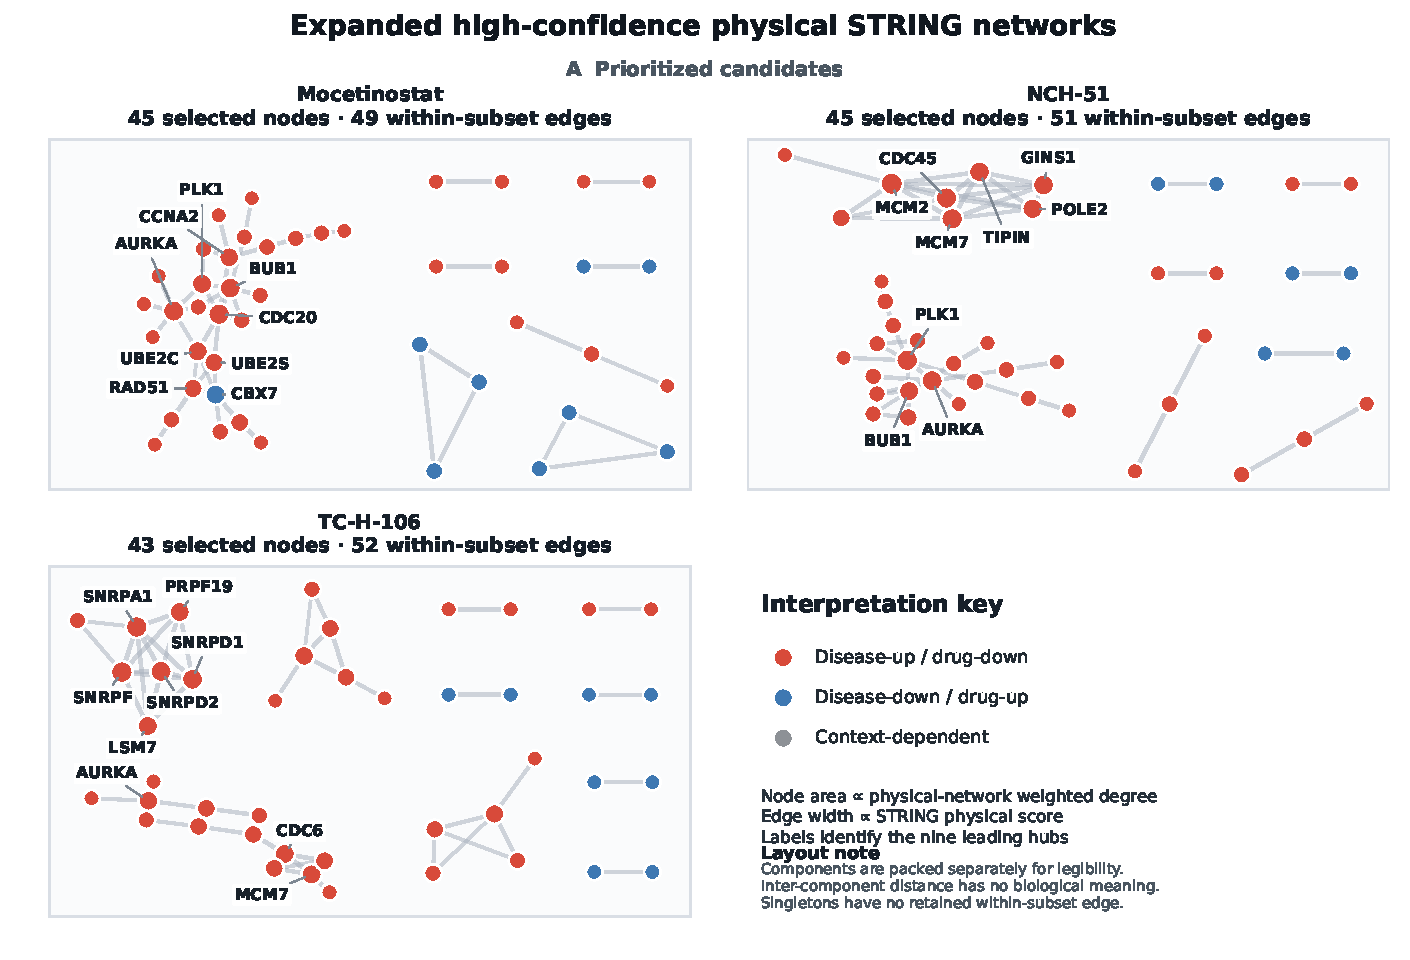
\includegraphics[page=1,height=5.55in,keepaspectratio]{supplementary_expanded_physical_networks.pdf}
\captionof{figure}{\textbf{(A) Expanded high-confidence physical STRING plotting subsets.} Mocetinostat, NCH-51, and TC-H-106 are shown with up to 45 non-isolated nodes selected by weighted degree. Leading hubs are labeled. Full 200-gene node tables and all physical/functional edges are in Additional file 2.}
\end{landscape}

\begin{landscape}
\centering
\includegraphics[page=2,height=5.55in,keepaspectratio]{supplementary_expanded_physical_networks.pdf}
\captionof*{figure}{\textbf{Supplementary Figure S4 (continued), panel B. Expanded high-confidence physical STRING plotting subsets for controls.} Belinostat, Entinostat, and Vorinostat are shown under the same plotting policy. Nodes remain reversal-associated genes, not direct drug targets.}
\end{landscape}

\section{DepMap genetic-dependency context}

\begingroup
\small
\begin{table}[H]
\centering
\caption{DepMap Public 26Q1 pan-cancer class I HDAC gene-effect summary.}
\label{tab:s_depmap}
\begin{tabular}{@{}lrrrrrr@{}}
\toprule
Gene & Models & Median & 95\% low & 95\% high & $\leq-0.5$ \% & $\leq-1.0$ \% \\
\midrule
HDAC1 & 1,208 & -0.107 & -0.118 & -0.093 & 4.5 & 1.1 \\
HDAC2 & 1,208 & 0.001 & -0.008 & 0.013 & 3.1 & 0.5 \\
HDAC3 & 1,208 & -1.215 & -1.249 & -1.188 & 95.1 & 68.2 \\
HDAC8 & 1,208 & -0.121 & -0.134 & -0.107 & 4.9 & 0.1 \\
\bottomrule
\end{tabular}
\end{table}
\endgroup
\begingroup
\small
\begin{table}[H]
\centering
\caption*{Supplementary Table S21 (continued). Lineage heterogeneity. Effect sizes are modest despite FDR significance.}
\begin{tabular}{@{}lrrrrrr@{}}
\toprule
Gene & Lineages & Models & Kruskal $H$ & $P$ & $\epsilon^2$ & FDR \\
\midrule
HDAC1 & 24 & 1,193 & 107.32 & 7.49e-13 & 0.072 & 1.50e-12 \\
HDAC2 & 24 & 1,193 & 119.95 & 4.24e-15 & 0.083 & 1.70e-14 \\
HDAC3 & 24 & 1,193 & 95.64 & 7.90e-11 & 0.062 & 1.05e-10 \\
HDAC8 & 24 & 1,193 & 71.71 & 6.61e-07 & 0.042 & 6.61e-07 \\
\bottomrule
\end{tabular}
\end{table}
\endgroup


HDAC3 is the dominant pan-cancer dependency in DepMap Public 26Q1. The lineage tests are statistically significant with modest effect sizes, and pairwise HDAC correlations are weak. These results provide genetic-loss context but do not identify a candidate's pharmacological isoform, efficacy, or normal-tissue safety.

\begin{landscape}
\centering
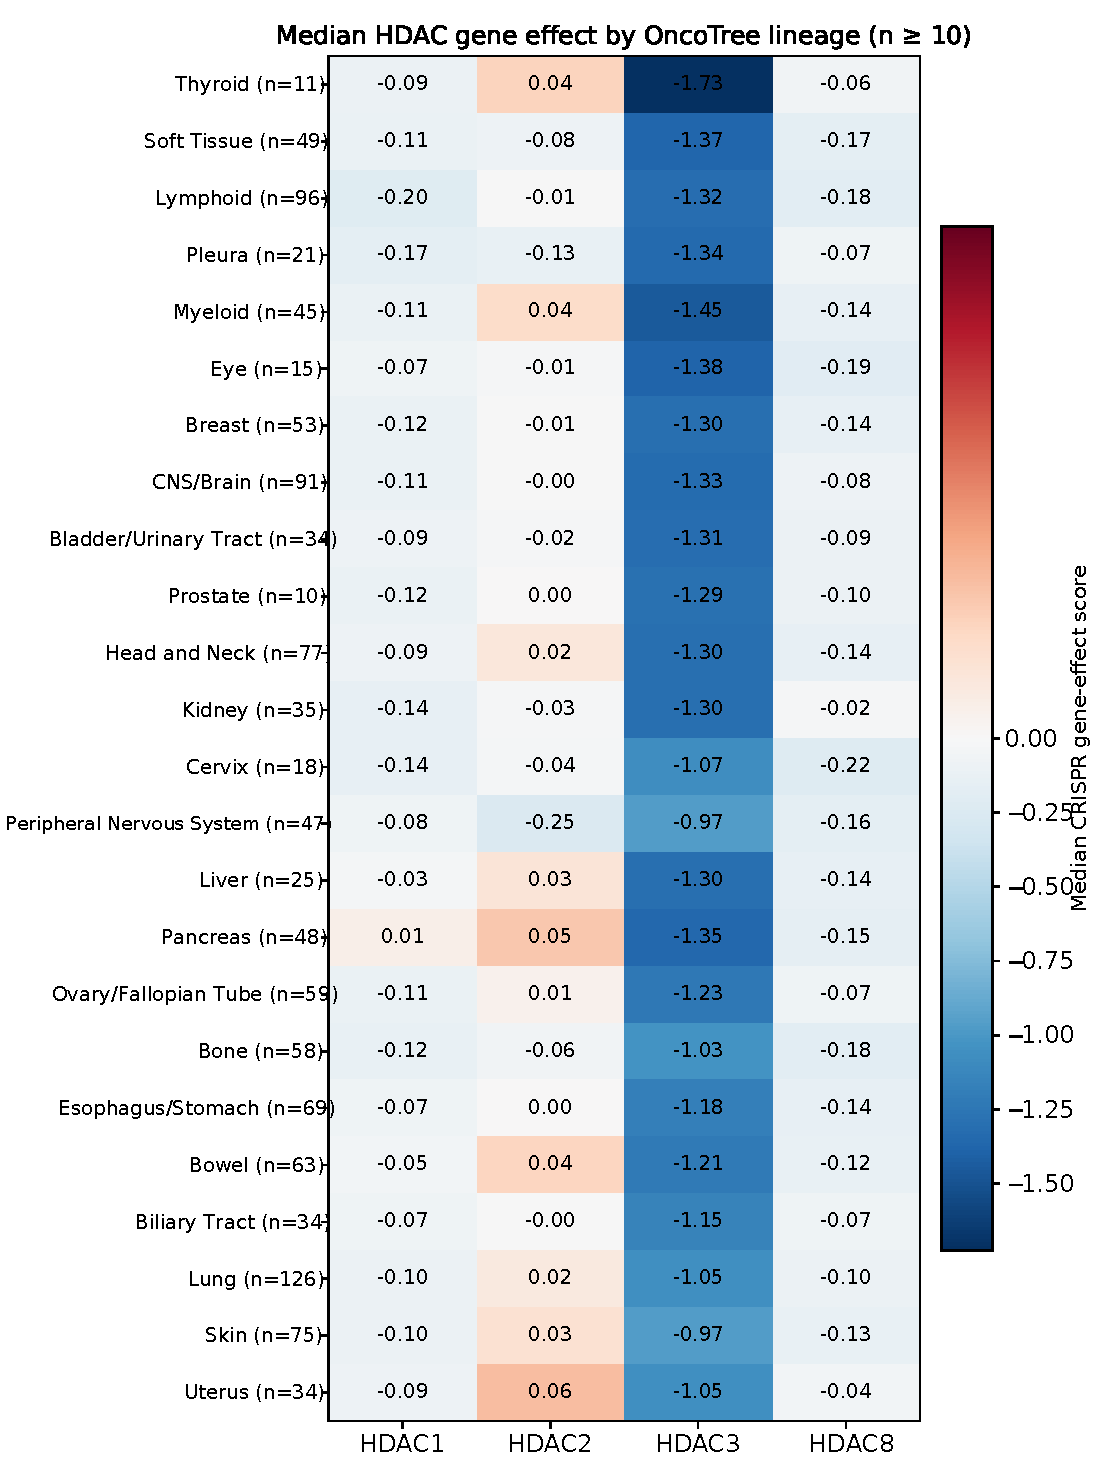
\includegraphics[height=5.45in,keepaspectratio]{depmap_hdac_lineage_heatmap.pdf}
\captionof{figure}{\textbf{DepMap lineage heterogeneity.} Median class I HDAC CRISPR gene effects are shown only for lineages meeting the prespecified minimum of ten models. More negative values indicate stronger loss-of-function effect.}
\end{landscape}

\begin{landscape}
\section{Controlled docking and receptor sensitivity}
\begingroup
\footnotesize
\begin{table}[H]
\centering
\caption{4LXZ crystallographic redocking control. The prespecified RMSD gate was 2 Angstrom.}
\label{tab:s_redock}
\begin{tabular}{@{}lrrrrrrr@{}}
\toprule
Method & Seeds & Seed coverage & Cluster poses & Median score & Medoid RMSD & Zn min & Zn max \\
\midrule
vina\_standard & 3 & 3 & 8 & -7.290 & 4.771 & 2.348 & 3.645 \\
ad4zn & 3 & 3 & 3 & -7.491 & 1.091 & 2.123 & 3.108 \\
\bottomrule
\end{tabular}
\end{table}
\endgroup
\begingroup
\scriptsize
\begin{table}[H]
\centering
\caption*{Supplementary Table S22 (continued). Frozen 4LXZ control/candidate panel. Favorable score is not evidence of intended zinc geometry.}
\begin{tabular}{@{}p{3.2cm}p{6.0cm}rrrrrrr@{}}
\toprule
Compound & Role & 3-seed & Poses & Cluster score & Medoid score & ZBG min & ZBG max & Nearest heteroatom \\
\midrule
Vorinostat & crystallographic\_positive\_control & yes & 3 & -7.491 & -7.532 & 2.123 & 3.108 & 2.123 \\
Vorinostat O-methyl decoy & designed zinc-chelation sensitivity control & yes & 6 & -7.998 & -7.791 & 6.799 & 8.992 & 4.078 \\
Mocetinostat & core\_candidate & yes & 7 & -11.024 & -12.289 & 12.954 & 13.872 & 2.002 \\
NCH-51 & secondary\_candidate & yes & 8 & -8.357 & -9.094 & -- & -- & 2.448 \\
TC-H-106 & original\_method\_sensitive\_candidate & yes & 5 & -9.674 & -9.895 & 10.442 & 13.748 & 3.858 \\
Entinostat & reference\_control & yes & 10 & -10.703 & -11.996 & 11.852 & 13.867 & 1.918 \\
Belinostat & class\_support\_control & yes & 3 & -9.336 & -9.383 & 8.918 & 9.525 & 2.841 \\
\bottomrule
\end{tabular}
\end{table}
\endgroup
\begingroup
\footnotesize
\begin{table}[H]
\centering
\caption*{Supplementary Table S22 (continued). HDAC2 4LXZ versus aligned HDAC1 4BKX receptor sensitivity.}
\begin{tabular}{@{}lrrrrrr@{}}
\toprule
Compound & Pose RMSD & 4LXZ score & 4BKX score & $\Delta$ score & 4LXZ nearest Zn & 4BKX nearest Zn \\
\midrule
Vorinostat & 8.357 & -7.491 & -8.111 & -0.620 & 2.123 & 2.324 \\
Vorinostat O-methyl decoy & 1.872 & -7.998 & -7.767 & 0.231 & 4.078 & 2.210 \\
Mocetinostat & 1.080 & -11.024 & -10.864 & 0.160 & 2.002 & 2.176 \\
NCH-51 & 1.870 & -8.357 & -8.457 & -0.100 & 2.448 & 2.435 \\
TC-H-106 & 1.508 & -9.674 & -8.886 & 0.788 & 3.858 & 3.895 \\
Entinostat & 1.280 & -10.703 & -10.539 & 0.164 & 1.918 & 1.907 \\
Belinostat & 8.787 & -9.336 & -7.915 & 1.421 & 2.841 & 2.140 \\
\bottomrule
\end{tabular}
\end{table}
\endgroup


\begin{minipage}{0.96\linewidth}
\small
The redocking control establishes protocol suitability only for one known cocrystal geometry under the zinc-aware potential. The O-methyl decoy demonstrates that a favorable score can coexist with an implausible prespecified zinc-binding-group distance. Several candidate poses change across 4LXZ and 4BKX. Consequently, docking is a protocol/receptor-sensitivity analysis with unresolved pose plausibility, not binding validation.
\end{minipage}
\end{landscape}

\begin{landscape}
\centering
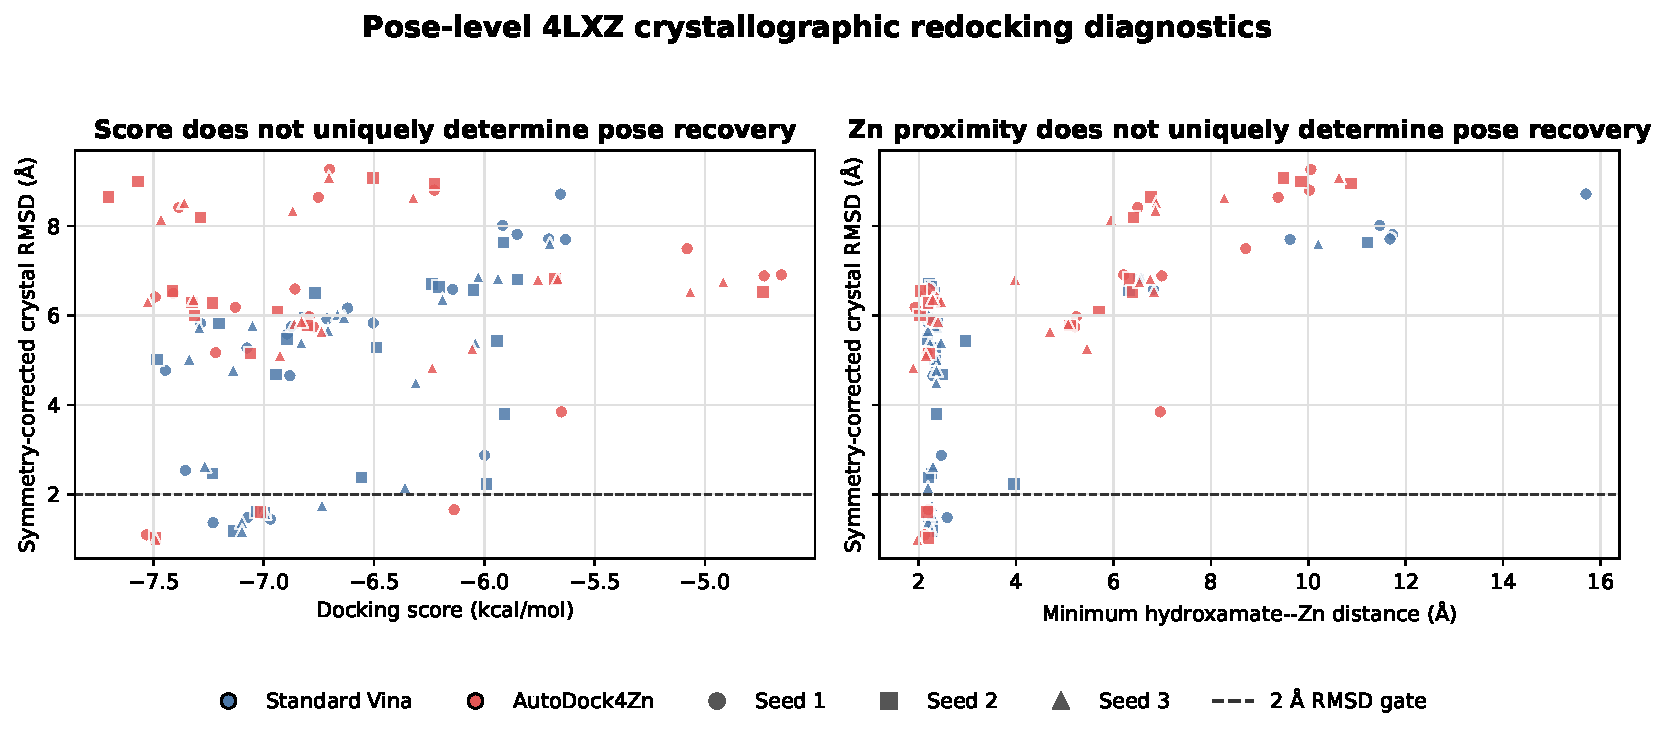
\includegraphics[width=0.96\linewidth,keepaspectratio]{redocking_pose_diagnostics.pdf}
\captionof{figure}{\textbf{Pose-level crystallographic redocking diagnostics.} Every retained pose from seeds 1--3 is shown by docking method. Score, symmetry-corrected heavy-atom RMSD, and hydroxamate--zinc distance are displayed jointly with the prespecified 2~\AA{} RMSD gate. These pose-level diagnostics expand main Figure 9 and show why score or zinc proximity alone cannot establish a recovered binding geometry.}
\end{landscape}

\section{External drug-sensitivity availability and reproducibility}

\begingroup
\footnotesize
\begin{table}[H]
\centering
\caption{External direct drug-sensitivity availability and null results. The public-transcriptomic option was completed; no surrogate is presented as direct validation.}
\label{tab:s_external}
\begin{tabular}{@{}p{0.13\textwidth}p{0.17\textwidth}p{0.21\textwidth}p{0.14\textwidth}p{0.22\textwidth}@{}}
\toprule
Scope & Endpoint & Availability & Result & Interpretation \\
\midrule
TC-H-106 & Direct public viability response & Unavailable in frozen public-data audit & Not performed & No direct external drug-sensitivity validation claimed \\
Entinostat & GDSC surrogate correlation & Available but not candidate matched & Pearson R=-0.052; P=0.859 & Null result; cannot validate TC-H-106 \\
All frozen candidates & New wet-lab viability/biochemical assay & Not performed; reviewer suggested wet-lab assays or public transcriptomic validation & Official-condition measured LINCS used as the public transcriptomic option & Does not replace viability or biochemical validation \\
\bottomrule
\end{tabular}
\end{table}
\endgroup


The non-significant Entinostat surrogate result is retained as a null result and cannot validate TC-H-106. No direct candidate-matched public viability response was found for TC-H-106 in the frozen audit. This limitation is stated in the manuscript and response letter rather than replaced with a post hoc proxy.

\input{generated/table_S24}

CPU model and RAM were not captured in the frozen AutoDL manifests. They are explicitly marked unrecorded rather than inferred from the current environment. The corrected evidence snapshot is archived at repository commit \texttt{fefbf2f4fa7399983d4d4041dcb8e7e91b84d17f}; later document-only commits do not alter that frozen analysis snapshot.

\section{Machine-readable companion}

Additional file 2 contains the complete preserved run-level, candidate-level, network, pathway, DepMap, docking, sensitivity, and reproducibility tables with filters and a data dictionary. A TCGA cohort manifest identifies all 22 GDC projects and the frozen disease-matrix hashes; per-cohort final tumor/normal counts were not retained and are not retrospectively reconstructed. A separate condition-level manifest records the schema of the analysis-time 83,490-row table and explicitly discloses that the source file and its SHA256 were not preserved in the frozen portable package. All preserved aggregates used for the reported figures and inferences are included. Repository-relative source paths are used; no AutoDL absolute paths are required to interpret the workbook. Blank fields are retained only when a measurement is not applicable or was not recorded, and the corresponding reason is supplied in a status or note column.

\end{document}
